%% For Slides
\documentclass[xcolor=x11names,compress,mathserif]{beamer}
%% For handouts
%\documentclass[xcolor=x11names,compress,mathserif,12pt,handout]{beamer}
%% To put multiple pages (say 2x3) per page in pdf,  use command 
%% pdfnup --a4paper --keepinfo --nup 2x3 --frame true \
%%      --scale 0.95 --no-landscape --outfile handout.pdf <input>.pdf
%% End of For Handout

\usepackage{etex}
%% Beamer Layout %%%%%%%%%%%%%%%%%%%%%%%%%%%%%%%%%%
\useoutertheme[subsection=false,shadow]{miniframes}
\useinnertheme{default}
\usefonttheme{structureitalicserif}
\usepackage{palatino}
%% packages from the paper
\usepackage{schemepgm}
\usepackage{graphicx}
\usepackage{mathrsfs}
\usepackage{graphpap}
\usepackage{tabularx}
\usepackage{epsfig}
\usepackage{pstricks}
\usepackage{pst-text}
\usepackage{pst-node}
\usepackage{pst-tree}
\usepackage{pst-rel-points}
\usepackage{boxedminipage}
\usepackage{algorithmic}
\usepackage{amssymb}
\usepackage{amsmath}
%%%%%%%%%% IMPERATIVE %%%%%%%%%%%%

%%%%%%%%%%%%%%%%%%%%%%%%%%%%%%%%%%%%%%%%%%%%%%%%%%%%%%%%%%%%%%%%%%
%%% Comment out a part of latex document
\newcommand{\cmt}[1]{}
\newcommand{\akadd}[1]{\protect{\red  #1}}
\newcommand{\akdel}[1]{\protect{\blue #1}}
\newcommand{\del}[1]{\protect{\magenta #1}}

\newcommand{\mybox}{\hfill\ensuremath{\Diamond}}
\newcommand{\NDIn}[1]{\mbox{\sf In$_#1$}}
\newcommand{\NDOut}[1]{\mbox{\sf Out$_#1$}}
%\newcommand{\x}{\cx}
%\newcommand{\y}{\cy}
%%%%%%%%%%%%%%%%%%%%%%%%%%%%%%%%%%%%%%%%%%%%%%%%%%%%%%%%%%%%%%%%%%

%%%%%%%%%%%%%%%%%%%%%%%%%%%%%%%%%%%%%%%%%%%%%%%%%%%%%%%%%%%%%%%%%%
%%%% Programs in latex 
\protect{\newlength{\FTABL}}
\protect{\newlength{\TABL}}
\protect{\newlength{\BRACE}}
\settowidth{\BRACE}{\{}

%%%%%%%%%%%%%%%%%%%%%%%%%%%%%%%%%%%%%%%%%%%%%%%%%%%%%%%%%%%%%%%%%%

 \newcommand{\ntbar}{\ensuremath{\overline\nt}}
%% %%%%%%%%%%%%%%%%%%%%%%%%%%%%%%%%%%%%%%%%%%%%%%%%%%%%%%%%%%%%%%%%%%
%%% Special pictures
\newcommand{\myarrow}{\mbox{%
 \psset{unit=1cm}%
 \begin{pspicture}(0,0)(.27,.2)%
  \psline[linewidth=.15mm]%
  (0,.1)(.125,.1)(.125,.035)(.25,.1)(.125,.165)(.125,.1)%
  \end{pspicture}}%
} 



%%
%% paths and derefs
\newcommand{\epath}{\mathsf{ep}}
\newcommand{\paths}{{\sf paths}}
\newcommand{\dpaths}{{\sf dpaths}}
\newcommand{\Pf}[2]{\ensuremath{\Pfonly_{\!\!#1}^{\,#2}}}
\newcommand{\Pfonly}{\ensuremath{\mathsf{PF}}}
\newcommand{\Pp}[2]{\ensuremath{\Pponly_{\!\!#1}^{\,#2}}}
\newcommand{\Pponly}{\ensuremath{\mathsf{PP}}}
\newcommand{\Pe}[3]{\ensuremath{\Peonly(#1, #2, #3)}}
\newcommand{\Peonly}{\ensuremath{\mathsf{PE}}}
\newcommand{\Peb}[3]{\ensuremath{\Pebonly(#1, #2, #3)}}
\newcommand{\Pebonly}{\ensuremath{\Peonly!}}
\newcommand{\Pv}{\ensuremath{\mathsf{P}}}
\newcommand{\Pvphi}{\ensuremath{\Pv^\emptyset}}
\newcommand{\Ddf}[2]{\ensuremath{\Ddfonly_{\!\!#1}^{\,#2}}}
\newcommand{\Ddfonly}{\ensuremath{\mathsf{DF}}}
\newcommand{\Dp}[2]{\ensuremath{\Dponly_{\!\!#1}^{\,#2}}}
\newcommand{\Dponly}{\ensuremath{\mathsf{DP}}}
\newcommand{\De}[3]{\ensuremath{\Deonly(#1, #2, #3)}}
\newcommand{\Deonly}{\ensuremath{\mathsf{DE}}}
%%\newcommand{\Deb}[3]{\ensuremath{\Debonly(#1, #2, #3)}}
%%\newcommand{\Debonly}{\ensuremath{\Deonly!}}
\newcommand{\Dv}{\ensuremath{\mathsf{D}}}
\newcommand{\Dvphi}{\ensuremath{\Dv^\emptyset}}
\newcommand{\derefs}{{\sf derefs}}

\newcommand{\bw}[1]{\ensuremath{\overline{#1}}} % backward
\newcommand{\cat}[2]{\ensuremath{#1#2}} % concat
\newcommand{\expshare}{\ensuremath{\mathsf{ExpS}}} % generic path

%% heap location and heap cell
\newcommand{\loc}[1]{\ensuremath{\mbox{\sf Loc}[{#1}]}}
\newcommand{\cell}[1]{\ensuremath{\mbox{\sf Cell}[{#1}]}}

%% type of labels
\newcommand{\acar}{\ensuremath{\mathbf{0}}}
\newcommand{\acdr}{\ensuremath{\mathbf{1}}}
\newcommand{\bcar}{\ensuremath{\bar\acar}}
\newcommand{\bcdr}{\ensuremath{\bar\acdr}}
\newcommand{\clazy}{\ensuremath{{\mathbf{2}}}}
\newcommand{\bX}  {\ensuremath{\bar{X}}}
\newcommand{\acarset}{\ensuremath{\lbrace\acar\rbrace}}
\newcommand{\acdrset}{\ensuremath{\lbrace\acdr\rbrace}}
\newcommand{\bcarset}{\ensuremath{\lbrace\bcar\rbrace}}
\newcommand{\bcdrset}{\ensuremath{\lbrace\bcdr\rbrace}}
\newcommand{\epsilonset}{\ensuremath{\lbrace\epsilon\rbrace}}

%%  transfer eqns - alias
\newcommand{\Af}[2]{\ensuremath{\Afonly_{#1}^{\,#2}}}
\newcommand{\Afonly}{\ensuremath{\mathsf{SF}}}
\newcommand{\Ap}[2]{\ensuremath{\Aponly_{#1}^{\,#2}}}
\newcommand{\Aponly}{\ensuremath{\mathsf{SP}}}
\newcommand{\Ae}[3]{\ensuremath{\Aeonly(#1, #2, #3)}}
\newcommand{\Aeonly}{\ensuremath{\mathsf{SE}}}
\newcommand{\Aa}[2]{\ensuremath{\Aaonly(#1, #2)}}
\newcommand{\Aaonly}{\ensuremath{\mathsf{SS}}}
\newcommand{\Av}{\ensuremath{\mathsf{S}}}
\newcommand{\Aphi}{\ensuremath{\Av^\emptyset}}
\newcommand{\Dfonly}{\ensuremath{\mathsf{D}}}
\newcommand{\Ufonly}{\ensuremath{\mathsf{I}}}
%\newcommand{\calls}[2]{\ensuremath{{\mathit{\!c}_{{\mathit #1}_#2}}}}
\newcommand{\calls}[2]{\ensuremath{{\mathit{\!c}_{{\mathit #1}}^#2}}}
%%\newcommand{\calls}[2]{\ensuremath{{\overline{\mathit #1}_{#2}}}}
%%  transfer eqns - liveness
\newcommand{\Uf}[2]{\ensuremath{\mathsf{I}_{\mathit #1}^{#2}}}
\newcommand{\Lfun}[3]{\ensuremath{\mathcal{L}(#1,#2,#3)}}
\newcommand{\Lfunonly}{\ensuremath{\mathcal{L}}}

\newcommand{\Df}[2]{\ensuremath{\mathsf{D}_{\mathit #1}^{#2}}}


\newcommand{\Lf}[3]{\ensuremath{\Lfonly_{\mathit #1}^{#2}( {\mathit #3})}}
\newcommand{\Lfonly}{\ensuremath{\mathsf{LF}}}
\newcommand{\Lfone}[1]{\ensuremath{\Lfonly_{\mathit #1}}}
\newcommand{\Le}[1]{\ensuremath{\Leonly({\mathit #1})}}
\newcommand{\Leonly}{\ensuremath{\mathsf{LE}}}
\newcommand{\Lp}[2]{\ensuremath{\Lponly_{#1}^{\,#2}}}
\newcommand{\Lponly}{\ensuremath{\mathsf{LP}}}
\newcommand{\Ld}[3]{\ensuremath{\Ldonly_{\mathit #1}^{#2}( {\mathit #3})}}
\newcommand{\Ldonly}{\ensuremath{\mathsf{LD}}}
\newcommand{\Lvc}[2]{\ensuremath{\Lv_{\mathit #1}^{\mathit #2}}}

\newcommand{\Lv}{\ensuremath{\mathsf{L}}}
\newcommand{\Lvphi}{\ensuremath{\Lv^\emptyset}}
\newcommand{\Leb}[3]{\ensuremath{\Lebonly(#1, #2, #3)}}
\newcommand{\Lebonly}{\ensuremath{\Leonly!}}
\newcommand{\NFA}{\mbox{\sf nfa}}
\newcommand{\lang}[1]{\ensuremath{\mathscr{L}({#1})}}
\newcommand{\Lan}[1]{\ensuremath{\Lv_{{#1}}}}
\newcommand{\Lanv}[2]{\ensuremath{\Lv_{{#1}}^{#2}}}
\newcommand{\dfa}[2]{\ensuremath{\mathsf{dfa}_{{#1}}^{#2}}}
%%  transfer eqns - availability
\newcommand{\AVf}[2]{\ensuremath{\AVfonly_{#1}^{\,#2}}}
\newcommand{\AVfonly}{\ensuremath{\mathsf{AvF}\,}}
\newcommand{\AVp}[2]{\ensuremath{\AVponly_{#1}^{\,#2}}}
\newcommand{\AVponly}{\ensuremath{\mathsf{AvP}\,}}
\newcommand{\AVgp}[2]{\ensuremath{\AVgponly_{#1}^{\,#2}}}
\newcommand{\AVgponly}{\ensuremath{{\mathsf{AvBP}}}}
\newcommand{\AVgf}[2]{\ensuremath{\AVgfonly_{#1}^{\,#2}}}
\newcommand{\AVgfonly}{\ensuremath{{\mathsf{AvBF}\,}}}
\newcommand{\AVe}[3]{\ensuremath{\AVeonly(#1, #2, #3)}}
\newcommand{\AVeonly}{\ensuremath{\mathsf{AvE}\,}}
\newcommand{\AVv}{\ensuremath{\mathsf{AV}}}
%\newtheorem{observation}[theorem]{Observation}

%%  transfer eqns - anticipability
\newcommand{\ANf}[2]{\ensuremath{\ANfonly_{#1}^{\,#2}}}
\newcommand{\ANfonly}{\ensuremath{\mathsf{AnF}}}
\newcommand{\ANp}[2]{\ensuremath{\ANponly_{#1}^{\,#2}}}
\newcommand{\ANponly}{\ensuremath{\mathsf{AnP}}}
\newcommand{\ANgp}[2]{\ensuremath{\ANgponly_{#1}^{\,#2}}}
\newcommand{\ANgponly}{\ensuremath{{\mathsf{AnBP}}}}
\newcommand{\ANgf}[2]{\ensuremath{\ANgfonly_{#1}^{\,#2}}}
\newcommand{\ANgfonly}{\ensuremath{{\mathsf{AnBF}}}}
\newcommand{\ANe}[3]{\ensuremath{\ANeonly(#1, #2, #3)}}
\newcommand{\ANeonly}{\ensuremath{\mathsf{AnE}}}
\newcommand{\ANv}{\ensuremath{\mathsf{AN}}}
\newcommand{\ANvphi}{\ensuremath{\ANv^\emptyset}}
\newcommand{\mmap}[3]{\ensuremath{\mathcal{M}_{\mathit{#1}}(\mathit{#2})(\mathit{#3})}}
\newcommand{\pmap}[1]{\ensuremath{\mathcal{P}_{\mathit{#1}}}}
\newcommand{\deltacall}[3]{\delta_{#1}({#2},{#3})}
%% union?
\newcommand{\plus}{$\cup$}

%% -> arrows, =def
\newcommand{\rightk}[1]{\ensuremath{\stackrel{\scriptstyle #1}{\rightarrow}}}
\newcommand{\rightstar}{\rightk{\star}}
%\newcommand{\eqdef}{\ensuremath{\stackrel{\scriptstyle def}{=}}}
\newcommand{\eqdef}{\ensuremath{=}}

%% functions

\newcommand{\listc}{\mbox{\tt l}}
\newcommand{\lista}{\mbox{\tt l1}}
\newcommand{\listb}{\mbox{\tt l2}}

%% nfa and cfg
\newcommand{\nfa}{\ensuremath{\mathbf{N}}}
\newcommand{\nfabar}{\ensuremath{\overline\nfa}}

\newcommand{\start}{{\sf init}}
\newcommand{\prim}{\ensuremath{P}}
\newcommand{\exit}{{\sf pgm}}
\newcommand{\gram}{\ensuremath{G}}
\newcommand{\nt}{\ensuremath{N}}
\newcommand{\var}[1]{\ensuremath{\langle #1\rangle}}

\newcommand{\TwoCells}[2]{%
\psset{unit=.25mm}
\begin{pspicture}(0,-2)(36,18)
\psframe(0,-5)(36,15)
\psline(18,-4)(18,15)
\putnode{zarb1342}{origin}{9}{5}{\rnode{#1}{}}
\putnode{zarb0102}{origin}{27}{5}{\rnode{#2}{}}
\end{pspicture}%
}

\newcommand{\TwoCellNull}[2]{%
\psset{unit=.25mm}
\begin{pspicture}(0,-2)(36,18)
\psframe(0,-5)(36,15)
\psline(18,-4)(18,15)
\psline(18,-4)(36,15)
\putnode{z}{origin}{9}{5}{\rnode{#1}{}}
\putnode{z}{origin}{27}{5}{\rnode{#2}{}}
\end{pspicture}%
}

\newcommand{\TwoCellsD}[2]{%
\psset{unit=.25mm}
\begin{pspicture}(0,-2)(36,18)
\psframe(0,-5)(36,15)
\psline(18,-4)(18,15)
\putnode{z}{origin}{9}{5}{\rnode{#1}{}}
\putnode{z}{origin}{27}{5}{\rnode{#2}{}}
\putnode{z}{origin}{9}{5}{%
      \psframebox[linestyle=none,fillstyle=hlines,hatchsep=2,framesep=8,
      hatchcolor=blue]{}}
\end{pspicture}%
}
\newcommand{\TwoCellsA}[2]{%
\psset{unit=.25mm}
\begin{pspicture}(0,-2)(36,18)
\psframe(0,-5)(36,15)
\psline(18,-4)(18,15)
\putnode{z}{origin}{9}{5}{\rnode{#1}{}}
\putnode{z}{origin}{9}{5}{%
   \psframebox[linestyle=none,fillstyle=hlines,hatchsep=2,framesep=8,
   hatchcolor=blue]{}}
\putnode{z}{origin}{27}{5}{\rnode{#2}{}}
\end{pspicture}%
}
\newcommand{\TwoCellsAD}[2]{%
\psset{unit=.25mm}
\begin{pspicture}(-6,-2)(42,18)
%\psframe(0,-5)(36,15)
%\psline(18,-4)(18,15)
\putnode{z}{origin}{9}{5}{\rnode{#1}{}}
\putnode{z}{origin}{9}{5}{%
   \psframebox[linestyle=none,fillstyle=solid,framesep=8,
   fillcolor=lightgray]{}}
\putnode{z}{origin}{27}{5}{%
      \psframebox[linestyle=none,fillstyle=solid,framesep=8,
   fillcolor=lightgray]{}}
\psccurve[fillstyle=solid,fillcolor=lightgray,linecolor=black]
(0,-5)(-6,5)(0,15)(12,20)(24, 15)(30,17)(36,15)(42,5)(36,-5)(24, -10)(12, -5)(6, -8)
\end{pspicture}%
}
% meta scheme command
\newcommand{\MIF}{\mbox{$\mathsf{if}$}}
\newcommand{\MEQ}{\mbox{$\mathsf{eq?}$}}
\newcommand{\MLET}{\mbox{$\mathsf{let}$}}
\newcommand{\MIN}{\mbox{$\mathsf{in}$}} 
%\newcommand{\IF}{\mbox{$\mathsf{if}$}}
%\newcommand{\SLET}{\mbox{$\mathsf{let}$}}
%\newcommand{\SIN}{\mbox{$\mathsf{in}$}} 

% others..
\newcommand{\candidates}[1]{\ensuremath{\mbox{\sf Candidates}(#1)}}
\newcommand{\scvars}[1]{\ensuremath{\mathsf{ScopeVars}(#1)}}
\newcommand{\expvars}[1]{\ensuremath{\mathsf{FV}(#1)}}
\newcommand{\mainpgm}{\ensuremath{\mathbf{main}}}
\newcommand{\main}{\ensuremath{\mathbf{main}}}
\newcommand{\updateenv}[3]{{\sf update(#1, #2, #3)}}
\newcommand{\pair}[2]{(#1, #2)}

\newcommand{\pia}{\ensuremath{\pi_{a}}}
\newcommand{\pib}{\ensuremath{\pi_{b}}}


\newenvironment{minieqnarray}
{\begin{minipage}{\textwidth}\begin{eqnarray}}
{\end{eqnarray}\end{minipage}}

%%% EFFECTIVENESS OF GC 
\newcommand{\deltarch}{\mbox{%
 \ensuremath{\delta_{\mbox{\footnotesize\sf rch}}}}}
\newcommand{\deltagc}{\mbox{%
 \ensuremath{\delta_{\mbox{\footnotesize\sf gc}}}}}
\newcommand{\GCstructure}{{\tt GC\_structure}}
\newcommand{\GCflag}{{\tt GC\_flag}}
\newcommand{\CreateTime}{{\tt Create\_time}}
\newcommand{\UseTime}{{\tt Use\_time}}
\newcommand{\CollTime}{{\tt Collection\_time}}
\newcommand{\exectime}{\mbox{\sf  T}}

\newcommand{\manual}[1]{{\protect#1}}

%% Benchmark names
\newcommand{\silex}{\mbox{\tt silex}}
\newcommand{\lalr}{\mbox{\tt lalr}}
\newcommand{\eopl}{\mbox{\tt eopl}}
\newcommand{\prolog}{\mbox{\tt prolog}}
\newcommand{\sudoku}{\mbox{\tt sudoku}}
\newcommand{\cipher}{\mbox{\tt cipher}}

%% helpful definitions
%%\renewcommand{\citeNP}{\cite}
\newcommand{\figtwo}{figure*}
\newcommand{\capsize}{}
\newcommand{\figrule}{}
\newcommand{\figtworule}{}

%% scheme program vars/constants
%% \renewcommand{\px}{\mbox{$\mathbf{x}$}}
%% \renewcommand{\py}{\mbox{$\mathbf{y}$}}
%% \renewcommand{\pz}{\mbox{$\mathbf{z}$}}
%% \renewcommand{\pw}{\mbox{$\mathbf{w}$}}
%% \newcommand{\pthree}{\mbox{$\mathbf{3}$}}
%% \newcommand{\pfour}{\mbox{$\mathbf{4}$}}
%% \newcommand{\pfive}{\mbox{$\mathbf{5}$}}
%% \newcommand{\psix}{\mbox{$\mathbf{6}$}}
%% \newcommand{\ptwo}{\mbox{$\mathbf{2}$}}
%% \newcommand{\append}{\mbox{$\mathbf{append}$}}
%% \newcommand{\set}{\mbox{$\mathbf{set{\mbox{\rm \bf !}}}$}}
%% \newcommand{\setcar}{\mbox{$\mathbf{set{\mbox{\rm \bf -}}car{\mbox{\rm \bf !}}}$}}
%% \newcommand{\setcdr}{\mbox{$\mathbf{set{\mbox{\rm \bf -}}cdr{\mbox{\rm \bf !}}}$}}

%% other defs
\newcommand{\nullifiable}{\mbox{\sf Nullifiable}}
\newcommand{\properprefix}{\mbox{\sf ProperPrefix}}
\newcommand{\prefix}{\mbox{\sf  Prefix}}
\newcommand{\linknull}{{\sf LinkNullify}}
\newcommand{\pathnullify}{{\sf PathNullify}}
\newcommand{\nullins}{{\sf GenNullCode}}
\newcommand{\nullstatements}{\mbox{\sf null-statements}}
\newcommand{\isnull}{\mbox{\sf isnull}}
\newcommand{\mymark}{\mbox{\sf Mark}}
\newcommand{\sbegin}{\mbox{\sf BEGIN}}
\newcommand{\map}{\mbox{\sf map}}
\newcommand{\nullset}{\ensuremath{\mathsf{N}}}
\newcommand{\insnull}[2]{\mbox{$\mathsf{InsertNull(#1,#2)}$}}  
\newcommand{\insnullfn}{\mbox{$\mathsf{InsertNull}$}}   

\newcommand{\compnullfn}{\mbox{$\mathsf{Nullify}$}} 
\newcommand{\compnull}[2]{\compnullfn(#1, #2)}
\newcommand{\compnullpgm}[1]{\mbox{$\mathsf{Nullifypgm(#1)}$}}
\newcommand{\compnulldef}[1]{\mbox{$\mathsf{Nullifydef(#1)}$}}

\newcommand{\zz}{{\sf z}}
\newcommand{\yy}{{\sf y}}
\newcommand{\xx}{{\sf x}}
\newcommand{\ww}{{\sf w}}
\newcommand{\uu}{{\sf u}}
\newcommand{\aap}{{\sf a}}
\newcommand{\result}{{\sf result}}

%% \newtheorem{lemma}{Lemma}[section]
%% \newtheorem{example}{Example}[section]
%% \newtheorem{theorem}{Theorem}[section]
%% \newtheorem{definition}{Definition}[section]
%% \newtheorem{corollary}{Corollary}[section]
%% \newtheorem{property}{Property}[section]
%% \newcommand{\qed}{\hfill\nobreak \ifvmode \relax \else
%%   \ifdim\lastskip<1.5em \hskip-\lastskip
%%   \hskip1.5em plus0em minus0.5em \fi \nobreak
%%   \vrule height0.75em width0.5em depth0.25em\  fi}
\newcommand{\qed}{\hfill\ensuremath{\square}}
 \newenvironment{proof}[1][Proof]{\begin{trivlist}
 \item[\hskip \labelsep {\bfseries #1}]}{\hfill\qed\end{trivlist}}

\newcommand{\expr}[1]{\ensuremath{#1}}
%\newcommand{\pv}[1] {\mbox{\tt #1}}
\newcommand{\db}[1]{{\bf [\![}#1{\bf ]\!]}}
\newcommand{\nat}{I\!\!N}
\newcommand{\lenprime}{\ \vdash^{l'}\ }
\newcommand{\len}{\ \vdash^l\ }
\newcommand{\sen}{\ \vdash^s\ }
\newcommand{\fen}{\ \vdash^f\ }
\newcommand{\den}{\ \vdash^f\ }
\newcommand{\argsen}{\ \vdash^{args}\ }
\newcommand{\pen}{\ \vdash^p\ }
\newcommand{\fsen}{\ \vdash^{fs}\ }
\newcommand{\psen}{\ \vdash^{ps}\ }

\newcommand{\last}{\mbox{last}}
\newcommand{\rightmost}{\mbox{rightmost}}
\newcommand{\before}{\mbox{before}}
\newcommand{\befen}{\ \vdash^{\sf before}}
\newcommand{\lasten}{\ \vdash^{\sf last}}
\newcommand{\rmen}{\ \vdash^{\sf rightmost}}
\newcommand{\rhos}{\ensuremath{\red \rho_s}}
\newcommand{\pgmpt}[1]{\ensuremath{\red \pi_{#1}}}
\newcommand{\multireduct}{\ensuremath{\stackrel{+}{\longrightarrow}}}
\newcommand{\avrightarrow}{\ensuremath{\longrightarrow}}
\newcommand{\multireductav}{\ensuremath{\stackrel{+}{\avrightarrow}}}
\newcommand{\heap}{\ensuremath{H}}       % heap
\newcommand{\ppn}[2]{\ensuremath{#2}} % prog point
\newcommand{\pp}[2]{\ensuremath{#2}} % prog point
\newcommand{\lvintp}{\ensuremath{\zeta}}
\newcommand{\avintp}{\lvintp}
\newcommand{\locs}{\mbox{\tt locs}} 
\newcommand{\llv}{\ensuremath{\mathcal{L}}}
\newcommand{\aav}{\ensuremath{\mathcal{A}}}
\newcommand{\aan}{\ensuremath{\mathcal{N}}}
\newcommand{\gl}{\mbox{\em G}}




%% packages from the paper
\setbeamerfont{title like}{shape=\scshape}
\setbeamerfont{frametitle}{shape=\scshape}

\setbeamercolor*{lower separation line head}{bg=DeepSkyBlue4} 
\setbeamercolor*{normal text}{fg=black,bg=white} 
\setbeamercolor*{alerted text}{fg=red} 
\setbeamercolor*{example text}{fg=black} 
\setbeamercolor*{structure}{fg=black} 
 
\setbeamercolor*{palette tertiary}{fg=black,bg=black!10} 
\setbeamercolor*{palette quaternary}{fg=black,bg=black!10} 

\renewcommand{\(}{\begin{columns}}
\renewcommand{\)}{\end{columns}}
\newcommand{\<}[1]{\begin{column}{#1}}
\renewcommand{\>}{\end{column}}

%%%%%%%%%%%%%%%%%%%%%%%%%%%%%%%%%%%%%%%%%%%%%%%%%%
\begin{document}
%%%%%%%%%%%%%%%%%%%%%%%%%%%%%%%%%%%%%%%%%%%%%%%%%%%%%%
%%%%%%%%%%%%%%%%%%%%%%%%%%%%%%%%%%%%%%%%%%%%%%%%%%%%%%
\section{\scshape Motivation}
\begin{frame}
\title{Liveness-Based Garbage Collection}
\author{
        {\bf Amey Karkare}\\{\it Indian Institute of Technology, Kanpur}\\ \and
        \\ {\em Joint work with} \\
        {\bf Amitabha Sanyal, Prasanna Kumar, Rahul Asati}\\{\it Indian Institute of
          Technology, Bombay}\\ \and
        {\bf Alan Mycroft}\\{\it University of Cambridge}
}


\date{
	%% \begin{tikzpicture}[decoration=Koch curve type 2] 
	%% 	\draw[DeepSkyBlue4] decorate{ decorate{ decorate{ (0,0) -- (3,0)}}}; 
	%% \end{tikzpicture}  
	%% \\
	February 9th, 2016
}
\titlepage
\end{frame}

%%%%%%%%%%%%%%%%%%%%%%%%%%%%%%%%%%%%%%%%%%%%%%%%%%%%%%
%%%%%%%%%%%%%%%%%%%%%%%%%%%%%%%%%%%%%%%%%%%%%%%%%%%%%%
%% \begin{frame}{Outline of Talk}
%% \tableofcontents
%% \end{frame}

%%%%%%%%%%%%%%%%%%%%%%%%%%%%%%%%%%%%%%%%%%%%%%%%%%%%%%
%%%%%%%%%%%%%%%%%%%%%%%%%%%%%%%%%%%%%%%%%%%%%%%%%%%%%%
\begin{frame}{Ideal Garbage Collection}
  \begin{quote}
    \ldots garbage collection (GC) is a form of automatic memory management.  The  garbage  collector,  or  just collector,  attempts  to  reclaim
  garbage, or memory occupied by objects  that are {\red no longer in use} by
  the program. \ldots
  \end{quote}
  From Wikipedia\\ {\scriptsize \url{https://en.wikipedia.org/wiki/Garbage_collection_(computer_science)}}
\end{frame}

\begin{frame}{Real Garbage Collection}
  \begin{quote}
    \ldots All garbage collectors use some efficient {\red approximation to
    liveness}. In {tracing} garbage collection, the approximation is that
    an object can't be live unless it is {\red reachable}. In {reference
      counting}, the approximation is that an object can't be live unless
    it is {\red referenced}. 
    \ldots
  \end{quote}
  From Memory Management Glossary\\
  {\scriptsize \url{http://www.memorymanagement.org/glossary/g.html\#term-garbage-collection}}
\end{frame}

\begin{frame}{Liveness based GC}
    \begin{itemize}\itemsep0.75em
    \item During execution, there are significant amounts of heap allocated data
      that  are {\em  reachable but not live}.
      \begin{itemize}
      \item Current GCs will retain such data.
      \end{itemize}
    \item Our idea: 
      \begin{itemize}
      \item We do a liveness analysis and provide GCs with its result.
      \item Modify GCs to mark data for retention {\em only if it is live}.
      \end{itemize}
    \item Consequences:
      \begin{itemize}
      \item  Fewer cells  marked.  \pause More  garbage collected  per
        collection. \pause Fewer garbage collections. \pause
      \item Programs expected to run faster and with smaller heap.
      \end{itemize}
    \end{itemize}
\end{frame}

%%%%%%%%%%%%%%%%%%%%%%%%%%%%%%%%%%%%%%%%%%%%%%%%%%%%%%
%%%%%%%%%%%%%%%%%%%%%%%%%%%%%%%%%%%%%%%%%%%%%%%%%%%%%%
\begin{frame}{An Example}
%%%%%%%%%%%%%%%%%%%%%%%%%%%%%%%%%%%%%%%%%%%%%%%%%%%%%%%%%%%%%%%%%%%%%%%%%%%
%%% MOTIVATING EXAMPLE

%%%%%%%%%%%%%%%%%%%%%%%%%%%%%%%%%%%%%%%%%%%%%%%%%%%%%%%%%%%%%%%%%%%%%%%%%%%
%%% MOTIVATING EXAMPLE
%% \newcommand{\nilfigure}
%% {\scalebox{0.75}{
%% \psset{unit=1mm,nodesep=0mm,labelsep=0.5mm}
%% \begin{pspicture}(0,0)(1,1)
%% %\psgrid[xunit=1cm,yunit=1cm,gridwidth=.2pt,subgridwidth=.1pt,subgriddiv=5,subgridcolor=gray,gridcolor=blue](0,0)(1,1)
%% \putnode{start}{origin}{0}{0}{}
%% \putnode{stop}{origin}{10}{10}{}
%% \ncline[offsetB=0,nodesepB=0,linewidth=.7]{-}{start}{stop} %here
%% \end{pspicture}
%% }}

%\begin{columns}
 % \begin{column}{0.5\textwidth}
%\begin{boxedminipage}{\textwidth}{
    \scalebox{0.75}{\sf
      \renewcommand{\arraystretch}{1}{
	\begin{uprogram}
	  \UFL\ \hspace*{-.31\TAL} (\DEFINE\ (\plength\  \lista)
	  \UNL{1}  (\SIF~(\NULLQ \ \lista)
	  0
	  \UNL{2}      ($+$\ 1\ (\plength\ (\CDR\  \lista)))))
          \UNL{2}
          \UNL{0}\ \hspace*{-.31\TAL} (\DEFINE\ (\pfun\  \listb)
	  \UNL{1}  ($+$\ 1\ (\CAR\  \listb)))
          %         \UNL{2}\;\;\;\;\;
          \UNL{0}
	  \UNL{0} \hspace*{-.49\TAL} $\pi_\mainpgm$ : (\LET\ \pz\   $\leftarrow$(\CONS\ ($+$\ $4$ $5$)\
          \UNL{0} \;\;\;\;\;\;\;\;\;\;\;\;\;\;\;\;\;\;\;\;\;\;\; (\CONS\ ($+$\ $5$ $2$) \NIL)) \IN
	  \UNL{0} \;\;\;\;\;\;\;\;\;\;\;\;(\SIF\ $*$\ 
	  \UNL{1} \;\;\;\;\;\;\;\;\;\;\;\; $\pi_1$: (\plength\ \pz\ )
	  \UNL{1} \;\;\;\;\;\;\;\;\;\;\;\; $\pi_2$: (\pfun\ \pz\ )))
	\end{uprogram}
  }}
%\end{boxedminipage}
  %% \end{column}
  %% \begin{column}{0.5\textwidth}
  %%   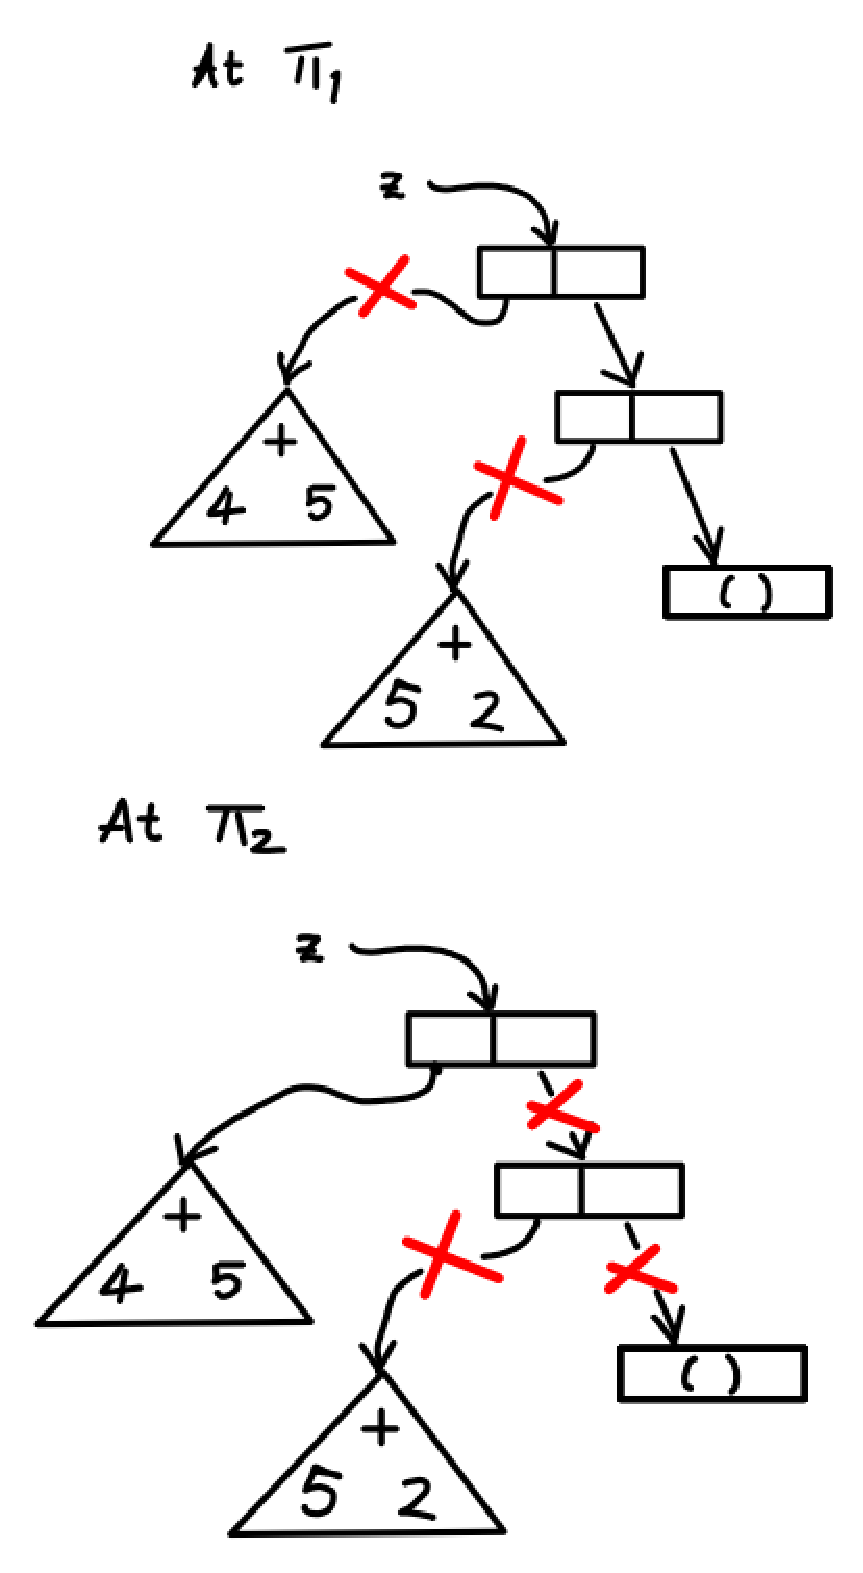
\epsfig{file=mem-graph.eps, height=6.5cm}
  %% \end{column}
%\end{columns}



\bigskip
\begin{itemize}
\item<1->{\em   Though    all   cells   are    reachable   at
  \rnode{A}{\red{$\pi$}},  a liveness-based  GC  will retain
  only  the cells  pointed by  thick  arrows.}  
\end{itemize}
\end{frame}

%%%%%%%%%%%%%%%%%%%%%%%%%%%%%%%%%%%%%%%%%%%%%%%%%%%%%%
%%%%%%%%%%%%%%%%%%%%%%%%%%%%%%%%%%%%%%%%%%%%%%%%%%%%%%
\section{\scshape Our method}

%% \begin{frame}{Liveness Information}
%%   \begin{itemize}
%%   \item Our analysis captures liveness as automata.
%%   \end{itemize}
%% \begin{columns}
%%   \begin{column}[T]{0.5\textwidth}
%% 

      \raisebox{-25mm}{\scalebox{.75}{
      \psset{unit=1mm}
      \psset{linewidth=.3mm}
      \begin{pspicture}(0,-5)(70,60)
%\psgrid[xunit=1cm,yunit=1cm,gridwidth=.2pt,subgridwidth=.1pt,subgriddiv=5,subgridcolor=gray,gridcolor=blue](0,-5)(7,6)
	%\psframe(0,0)(73,60)
	%%%%%%%%%%%%%%%%%%%%%%%%%%%%%%%%%%%%%%%%%%%%%%%%%%%%%%%%%%%%%%%%
	\putnode{y}{origin}{5}{40}{y}
        \putnode{nexty}{y}{13}{0}{}
        \ncline[nodesepB=1]{->}{y}{nexty}

	\putnode{z}{y}{0}{-12}{z}
        \putnode{nextz}{z}{13}{0}{}
        \ncline[nodesepB=1]{->}{z}{nextz}

	\putnode{w}{z}{0}{-12}{w}
        \putnode{state1}{w}{15}{0}{\pscirclebox[doubleline=true]{\ \ \ }}
        \ncline[nodesepB=-1.2]{->}{w}{state1}
         \putnode{state2}{state1}{15}{0}{\pscirclebox[doubleline=true]{\ \ \ }}
        \ncline[nodesepB=-1.2]{->}{state1}{state2}
       \aput(.5){\tt {\acdr}}
        \putnode{state3}{state2}{15}{0}{\pscirclebox[doubleline=true]{\
        \ \ }}
        \ncline[nodesepB=-1.2]{->}{state2}{state3}
        \aput(.5){\tt {\acar}}
        \nccurve[angleA=60,angleB=120,ncurv=5,nodesepA=-.2,nodesepB=-.7]{->}{state3}{state3}
%        \nccurve[angleA=0,angleB=0,nodesepB=-20]{->}{state3}{.4cm}
       \Bput[.1]{\tt {\acar\,$|$\!\!\! \acdr}}

        \putnode{cap}{w}{25}{-12}{\Large Liveness at \red{$\pi$}}

      \end{pspicture}}}


%%   \end{column}
%%   \begin{column}[T]{0.5\textwidth}
%%     

%%%%%%%%%%%%%%%%%%%%%%%%%%%%%%%%%%%%%%%%%%%%%%%%%%%%%%%%%%%%%%%%%%%%%%%%%%%
%%% MOTIVATING EXAMPLE
\newcommand{\nilfigure}
{\scalebox{0.75}{
\psset{unit=1mm,nodesep=0mm,labelsep=0.5mm}
\begin{pspicture}(0,0)(1,1)
%\psgrid[xunit=1cm,yunit=1cm,gridwidth=.2pt,subgridwidth=.1pt,subgriddiv=5,subgridcolor=gray,gridcolor=blue](0,0)(1,1)
\putnode{start}{origin}{0}{0}{}
\putnode{stop}{origin}{10}{10}{}
\ncline[offsetB=0,nodesepB=0,linewidth=.7]{-}{start}{stop} %here
\end{pspicture}
}}

 %%%%%%%%%%%%%%%%%%%%%%%%%%%%%%%%%%%%%%%%%%%%%%%%%%%%%%%%%%%%%%%%%%%%%%%%%%%
 %%% MOTIVATING EXAMPLE


       \raisebox{-25mm}{\scalebox{.65}{
         %%%%%%%%%%%%%%%%%%%%%Uday's stuff%%%%%%%%%%%%%%%%%%%%%%%%%
       \psset{unit=1mm}
       \psset{linewidth=.3mm}
       \begin{pspicture}(0,-5)(70,60)
% \psgrid[xunit=1cm,yunit=1cm,gridwidth=.2pt,subgridwidth=.1pt,subgriddiv=5,subgridcolor=gray,gridcolor=blue](0,-5)(7,6)
         %\psframe(0,0)(73,60)
         %%%%%%%%%%%%%%%%%%%%%%%%%%%%%%%%%%%%%%%%%%%%%%%%%%%%%%%%%%%%%%%%
         \putnode{o}{origin}{13}{50}{}%{\TwoCells{o1}{o2}}
         \putnode{a}{o}{-10}{-15}{\psframebox{3}}
%         \putnode{r}{origin}{26}{38}{}
%         \ncline[offsetB=-.5,nodesepB=.1]{*->}{o1}{a}
%         \putnode{b}{o}{0}{-3}{\psframebox[linestyle=none,framesep=.5]{\scalebox{.63}{\nilfigure}}}
 %	\ncline[offsetB=-.5,nodesepB=.1]{*->}{o2}{b}
         %\ncline[offsetB=-.5,nodesepB=.1]{->}{o2}{b}
%         \putnode{y}{o}{-14}{8}{\psframebox[linestyle=none,framesep=.5]{y}}
%        {\nccurve[nodesepB=-.2,angleA=330,angleB=120]{->}{y}{o}}
%         \aput[-3.5](.5){\scalebox{1.2}{\psframebox[framesep=.2,linestyle=none,fillstyle=solid,
%                   fillcolor=white]{$\times$}}}
         %%%%%%%%%%%%%%%%%%%%%%%%%%%%%%%%%%%%%%%%%%%%%%%%%%%%%%
         \putnode{c}{o}{25}{0}{\TwoCells{c1}{c2}}
         \putnode{d}{c}{10}{-10}{\TwoCells{d1}{d2}}
         \putnode{e}{d}{-13}{-12}{\TwoCells{e1}{e2}}
         \putnode{f}{d}{13}{-12}{\TwoCells{f1}{f2}}
%         \nccurve[nodesepB=-.2,angleA=330,angleB=120,linecolor=red]{->}{r}{e}
         \ncline[nodesepB=-.5]{*->}{c2}{d}
         \ncline[nodesepB=-.5,linewidth=.7]{->}{c2}{d}
         \nccurve[ncurv=1,angleA=180,angleB=0]{*->}{c1}{a}
         \aput[-3.5](.2){\scalebox{1.2}{\psframebox[framesep=.2,linestyle=none,fillstyle=solid,
               fillcolor=white]{$\times$}}}
         \nccurve[nodesepB=-.5,angleA=240,angleB=70,linecolor=red]{*->}{d1}{e}
         \nccurve[nodesepB=-.5,angleA=240,angleB=70,linewidth=.7,linecolor=red]{->}{d1}{e}
         \nccurve[nodesepB=-.5,angleA=300,angleB=110]{*->}{d2}{f}
         \aput[-3.5](.5){\scalebox{1.2}{\psframebox[framesep=.2,linestyle=none,fillstyle=solid,
               fillcolor=white]{$\times$}}}
         \putnode{w}{c}{-8}{8}{\psframebox[linestyle=none,framesep=.2]{w}}
 %        \putnode{ww}{c}{15}{8}{\psframebox[linestyle=none,framesep=.2]{z}}
         \nccurve[nodesepB=-.2,angleA=330,angleB=120,linewidth=.7]{->}{w}{c}
         %%%%%%%%%%%%%%%%%%%%%%%%%%%%%%%%%%%%%%%%%%%%%%%%%%%%%%%%%%%%%%%%%%
         \putnode{g}{e}{-8}{-12}{\psframebox{4}}
         \putnode{h}{e}{8}{-14}{\TwoCells{h1}{h2}}
         \putnode{i}{f}{-8}{-11}{\psframebox{6}}
 %	\putnode{j}{f}{8}{-11}{\psframebox[linestyle=none,framesep=.5]{\NIL}}
         \ncline[offsetB=-.5,nodesepB=.1]{*-}{e1}{e1}
         \ncline[linestyle=dashed,offsetB=-.5,nodesepB=.1,linewidth=.7]{->}{e1}{g}
         %here
         \putnode{j1}{f}{0}{-3}{\psframebox[linestyle=none,framesep=0]{\scalebox{.63}{\nilfigure}}}
         \putnode{j2}{h}{0}{-3}{\psframebox[linestyle=none,framesep=.5]{\scalebox{.63}{\nilfigure}}}

 %        \aput[-3.2](.6){\scalebox{1.2}{\psframebox[framesep=.1,linestyle=none,fillstyle=solid,
 %	      fillcolor=white]{$\times$}}} %and here
         \ncline[offsetB=-.5,nodesepB=-.3]{*-}{e2}{e2}
         \ncline[linestyle=dashed,offsetB=-.5,nodesepB=.1,linewidth=.7]{->}{e2}{h} 
 %	\aput[-3.2](.5){\scalebox{1.2}{\psframebox[framesep=.1,linestyle=none,fillstyle=solid,
 %	      fillcolor=white]{$\times$}}} %and here

         \ncline[offsetB=-.5,nodesepB=.1]{*->}{f1}{i}
         \ncline[offsetB=-.5,nodesepB=.1]{*->}{f2}{j}
         \nccurve[nodesepB=-.2,angleA=270,angleB=90]{->}{ww}{d}
         \aput[-3.2](.55){\scalebox{1.2}{\psframebox[framesep=.1,linestyle=none,fillstyle=solid,
               fillcolor=white]{$\times$}}}
         %%%%%%%%%%%%%%%%%%%%%%%%%%%%%%%%%%%%%%%%%%%%%%%%%%%%%%%%%%%%%%%%%%
         \putnode{k}{h}{-8}{-11}{\psframebox{5}}
 %	\putnode{l}{h}{8}{-11}{\psframebox[linestyle=none,framesep=.5]{\NIL}}
         \ncline[offsetB=-.5,nodesepB=.1]{*-}{h1}{h1}
         \ncline[linestyle=dashed,offsetB=-.5,nodesepB=.1,linewidth=.7]{->}{h1}{k}
 %	\ncline[offsetB=-.5,nodesepB=.1]{*->}{h2}{l}
         %%%%%%%%%%%%%%%%%%%%%%%%%%%%%%%%%%%%%%%%%%%%%%%%%%%%%%%%%%%%%%%%%%
       \end{pspicture}}} 



%%   \end{column}
%% \end{columns}
%% \end{frame}


%%%%%%%%%%%%%%%%%%%%%%%%%%%%%%%%%%%%%%%%%%%%%%%%%%%%%%
%%%%%%%%%%%%%%%%%%%%%%%%%%%%%%%%%%%%%%%%%%%%%%%%%%%%%%
\begin{frame}{The language analyzed}
\begin{columns}
  \begin{column}[T]{0.45\textwidth}
\small
    \begin{itemize} \itemsep0.75em
    \item First order eager Scheme-like functional language.
    \item In Administrative Normal Form (ANF).
%    \item The order  of
%      evaluation of function arguments is made explicit.
    \end{itemize}
\normalsize
  \end{column}
  \begin{column}[T]{0.55\textwidth}
    
\small
\begin{eqnarray*}
   p \in \mathit{Prog} & ::= & d_1 \ldots d_n \,\, e_\mainpgm \\
    d \in Fdef & ::= & (\DEFINE\,\, (f\,\, 
    x_1 \,\, \ldots \,\, x_n)\,\,
    e) 
    \hspace{1.7em} \mbox{} \\
e \in \mathit{Expr} & ::= &
\left\{\begin{array}{lll}
       (\SIF\,\, x\,\, e_1\,\, e_2) && \mbox{} \\  
       (\LET\,\, x \leftarrow a\,\, \IN\,\, e) && \mbox{} \\
       (\RETURN\,\, x) && \mbox{}
    \end{array}\right. \\
a \in \mathit{App} & ::= &
\left\{\begin{array}{lrl}
       k && \mbox{}\\
       (\CONS\,\, {\red x_1}\,\, {\red x_2}) && \mbox{} \\ 
       (\CAR\,\, {\red x)} &  (\CDR\,\, {\red x)} & \mbox{} \\ 
       (\NULLQ\,\, {\red x}) & (\PRIM\,\, {\red x_1}\,\, {\red x_2}) & \mbox{} \\ 
%        (\NULLQ\,\, x) && \mbox{\em ---  tester} \\ 
%       (\ID\,\, x) && \mbox{\em ---  identity function (for inlining)} \\ 
%        (\PRIM\,\, x_1\,\, x_2) && \mbox{\em --- generic arithmetic} \\ 
       \multicolumn{2}{l}{(f\,\,{\red  x_1}\,\,\ldots\,\, {\red x_n})} 
            & \mbox{} 
    \end{array}\right.
\end{eqnarray*}



  \end{column}
\end{columns}
\end{frame}


%%%%%%%%%%%%%%%%%%%%%%%%%%%%%%%%%%%%%%%%%%%%%%%%%%%%%%
%%%%%%%%%%%%%%%%%%%%%%%%%%%%%%%%%%%%%%%%%%%%%%%%%%%%%%
\section{\scshape Liveness}
\begin{frame}{Liveness -- Basic Concepts and Notations}
\small
\begin{columns}
  \begin{column}[T]{0.75\textwidth}
    \begin{itemize}\itemsep0.75em
    \item {\em Access paths:} Strings over \{\acar, \acdr\}.
      
      \hspace*{.25cm}   \acar\  -- access \CAR\ field \\
      \hspace*{.25cm}   \acdr\  -- access \CDR\ field 
    \item Denote traversals over the heap graph
    \item {\em Liveness environment:} 
      \only<1>
          {Maps root variables    to set of access paths.
            \begin{eqnarray*}
              \Lanv{i}{}&:&
              \left\{\begin{array}{l}
              y \mapsto \emptyset\\
              z \mapsto \{\epsilon\}\\
              w \mapsto \{\epsilon, 1, 10, 100\}
              \end{array}\right.
            \end{eqnarray*}
          }
          \only<2>
              {Alternate representation.
                \begin{eqnarray*}
                  \Lanv{i}{}&:&
                  \left\{\begin{array}{l}
                  \emptyset \;\; \cup  \\
                  \{z.\epsilon\} \;\; \cup\\
                  \{w.\epsilon, w.1, w.10, w.100\}
                  \end{array}\right.
                \end{eqnarray*} 
              }
    \end{itemize}
  \end{column}
  \begin{column}[T]{0.25\textwidth}
    \fbox{\centerline{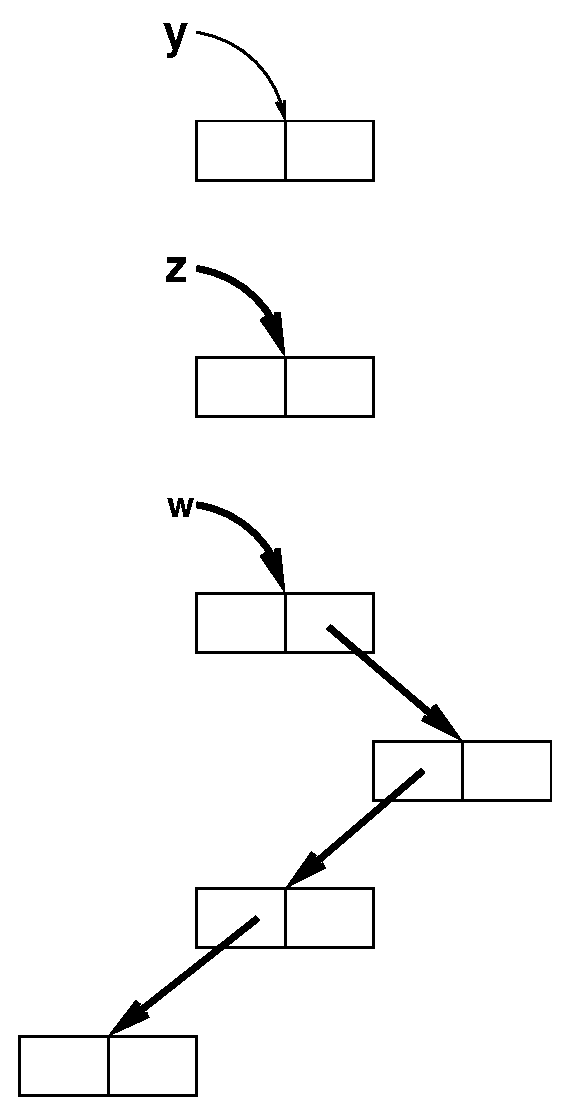
\epsfig{file=example-liveness-environment.eps, height=5cm}}}
  \end{column}
\end{columns}

\bigskip
\bigskip

\onslide<1>{Notation: We write \Lanv{i}{}(\px) as  \normalsize\Lanv{i}{\px}}
\end{frame}

%%%%%%%%%%%%%%%%%%%%%%%%%%%%%%%%%%%%%%%%%%%%%%%%%%%%%%
%%%%%%%%%%%%%%%%%%%%%%%%%%%%%%%%%%%%%%%%%%%%%%%%%%%%%%
\begin{frame}{Demand}
  \begin{center}
     (\CAR\ (\CDR\ \pw)) \\
  \end{center}
  \pause
\centerline{

%%%%%%%%%%%%%%%%%%%%%%%%%%%%%%%%%%%%%%%%%%%%%%%%%%%%%%%%%%%%%%%%%%%%%%%%%%%
%%% MOTIVATING EXAMPLE
\newcommand{\nilfigure}
{\scalebox{0.75}{
\psset{unit=1mm,nodesep=0mm,labelsep=0.5mm}
\begin{pspicture}(0,0)(1,1)
%\psgrid[xunit=1cm,yunit=1cm,gridwidth=.2pt,subgridwidth=.1pt,subgriddiv=5,subgridcolor=gray,gridcolor=blue](0,0)(1,1)
\putnode{start}{origin}{0}{0}{}
\putnode{stop}{origin}{10}{10}{}
\ncline[offsetB=0,nodesepB=0,linewidth=.7]{-}{start}{stop} %here
\end{pspicture}
}}

 %%%%%%%%%%%%%%%%%%%%%%%%%%%%%%%%%%%%%%%%%%%%%%%%%%%%%%%%%%%%%%%%%%%%%%%%%%%
 %%% MOTIVATING EXAMPLE


       \raisebox{-25mm}{\scalebox{.65}{
         %%%%%%%%%%%%%%%%%%%%%Uday's stuff%%%%%%%%%%%%%%%%%%%%%%%%%
       \psset{unit=1mm}
       \psset{linewidth=.3mm}
       \begin{pspicture}(0,-5)(70,60)
% \psgrid[xunit=1cm,yunit=1cm,gridwidth=.2pt,subgridwidth=.1pt,subgriddiv=5,subgridcolor=gray,gridcolor=blue](0,-5)(7,6)
         %\psframe(0,0)(73,60)
         %%%%%%%%%%%%%%%%%%%%%%%%%%%%%%%%%%%%%%%%%%%%%%%%%%%%%%%%%%%%%%%%
         \putnode{o}{origin}{13}{50}{}%{\TwoCells{o1}{o2}}
         \putnode{a}{o}{-10}{-15}{\psframebox{3}}
%         \putnode{r}{origin}{26}{38}{}
%         \ncline[offsetB=-.5,nodesepB=.1]{*->}{o1}{a}
%         \putnode{b}{o}{0}{-3}{\psframebox[linestyle=none,framesep=.5]{\scalebox{.63}{\nilfigure}}}
 %	\ncline[offsetB=-.5,nodesepB=.1]{*->}{o2}{b}
         %\ncline[offsetB=-.5,nodesepB=.1]{->}{o2}{b}
%         \putnode{y}{o}{-14}{8}{\psframebox[linestyle=none,framesep=.5]{y}}
%        {\nccurve[nodesepB=-.2,angleA=330,angleB=120]{->}{y}{o}}
%         \aput[-3.5](.5){\scalebox{1.2}{\psframebox[framesep=.2,linestyle=none,fillstyle=solid,
%                   fillcolor=white]{$\times$}}}
         %%%%%%%%%%%%%%%%%%%%%%%%%%%%%%%%%%%%%%%%%%%%%%%%%%%%%%
         \putnode{c}{o}{25}{0}{\TwoCells{c1}{c2}}
         \putnode{d}{c}{10}{-10}{\TwoCells{d1}{d2}}
         \putnode{e}{d}{-13}{-12}{\TwoCells{e1}{e2}}
         \putnode{f}{d}{13}{-12}{\TwoCells{f1}{f2}}
%         \nccurve[nodesepB=-.2,angleA=330,angleB=120,linecolor=red]{->}{r}{e}
         \ncline[nodesepB=-.5]{*->}{c2}{d}
         \ncline[nodesepB=-.5,linewidth=.7]{->}{c2}{d}
         \nccurve[ncurv=1,angleA=180,angleB=0]{*->}{c1}{a}
         \aput[-3.5](.2){\scalebox{1.2}{\psframebox[framesep=.2,linestyle=none,fillstyle=solid,
               fillcolor=white]{$\times$}}}
         \nccurve[nodesepB=-.5,angleA=240,angleB=70,linecolor=red]{*->}{d1}{e}
         \nccurve[nodesepB=-.5,angleA=240,angleB=70,linewidth=.7,linecolor=red]{->}{d1}{e}
         \nccurve[nodesepB=-.5,angleA=300,angleB=110]{*->}{d2}{f}
         \aput[-3.5](.5){\scalebox{1.2}{\psframebox[framesep=.2,linestyle=none,fillstyle=solid,
               fillcolor=white]{$\times$}}}
         \putnode{w}{c}{-8}{8}{\psframebox[linestyle=none,framesep=.2]{w}}
 %        \putnode{ww}{c}{15}{8}{\psframebox[linestyle=none,framesep=.2]{z}}
         \nccurve[nodesepB=-.2,angleA=330,angleB=120,linewidth=.7]{->}{w}{c}
         %%%%%%%%%%%%%%%%%%%%%%%%%%%%%%%%%%%%%%%%%%%%%%%%%%%%%%%%%%%%%%%%%%
         \putnode{g}{e}{-8}{-12}{\psframebox{4}}
         \putnode{h}{e}{8}{-14}{\TwoCells{h1}{h2}}
         \putnode{i}{f}{-8}{-11}{\psframebox{6}}
 %	\putnode{j}{f}{8}{-11}{\psframebox[linestyle=none,framesep=.5]{\NIL}}
         \ncline[offsetB=-.5,nodesepB=.1]{*-}{e1}{e1}
         \ncline[linestyle=dashed,offsetB=-.5,nodesepB=.1,linewidth=.7]{->}{e1}{g}
         %here
         \putnode{j1}{f}{0}{-3}{\psframebox[linestyle=none,framesep=0]{\scalebox{.63}{\nilfigure}}}
         \putnode{j2}{h}{0}{-3}{\psframebox[linestyle=none,framesep=.5]{\scalebox{.63}{\nilfigure}}}

 %        \aput[-3.2](.6){\scalebox{1.2}{\psframebox[framesep=.1,linestyle=none,fillstyle=solid,
 %	      fillcolor=white]{$\times$}}} %and here
         \ncline[offsetB=-.5,nodesepB=-.3]{*-}{e2}{e2}
         \ncline[linestyle=dashed,offsetB=-.5,nodesepB=.1,linewidth=.7]{->}{e2}{h} 
 %	\aput[-3.2](.5){\scalebox{1.2}{\psframebox[framesep=.1,linestyle=none,fillstyle=solid,
 %	      fillcolor=white]{$\times$}}} %and here

         \ncline[offsetB=-.5,nodesepB=.1]{*->}{f1}{i}
         \ncline[offsetB=-.5,nodesepB=.1]{*->}{f2}{j}
         \nccurve[nodesepB=-.2,angleA=270,angleB=90]{->}{ww}{d}
         \aput[-3.2](.55){\scalebox{1.2}{\psframebox[framesep=.1,linestyle=none,fillstyle=solid,
               fillcolor=white]{$\times$}}}
         %%%%%%%%%%%%%%%%%%%%%%%%%%%%%%%%%%%%%%%%%%%%%%%%%%%%%%%%%%%%%%%%%%
         \putnode{k}{h}{-8}{-11}{\psframebox{5}}
 %	\putnode{l}{h}{8}{-11}{\psframebox[linestyle=none,framesep=.5]{\NIL}}
         \ncline[offsetB=-.5,nodesepB=.1]{*-}{h1}{h1}
         \ncline[linestyle=dashed,offsetB=-.5,nodesepB=.1,linewidth=.7]{->}{h1}{k}
 %	\ncline[offsetB=-.5,nodesepB=.1]{*->}{h2}{l}
         %%%%%%%%%%%%%%%%%%%%%%%%%%%%%%%%%%%%%%%%%%%%%%%%%%%%%%%%%%%%%%%%%%
       \end{pspicture}}} 


}
  \begin{itemize}
  \item Demand  (notation: $\sigma$) is a description  of intended use
    of the result of an expression.
   \pause
\item We assume the demand on the main expression to be $(0+1)^*$,
  which we call $\sigma_{all}$.
\item The demands on each function body, $\sigma_f$, have to be computed.
  \end{itemize}



%% \bigskip

%% \begin{columns}
%%   \begin{column}{0.55\textwidth}
%% \centerline{$\sigma_{all} =  (0+1)^*$}
%% \input{demand-example}
%%   \end{column}
%%   \begin{column}{0.55\textwidth}
%%  
%%   \end{column}
%% \end{columns}
\end{frame}

%%%%%%%%%%%%%%%%%%%%%%%%%%%%%%%%%%%%%%%%%%%%%%%%%%%%%%
\begin{frame}[t]{Liveness analysis -- The big picture}

\setbeamercovered{transparent}
\small
\begin{columns}[c]
 \begin{column}[T]{0.5\textwidth}
\hspace*{-.3cm}\renewcommand{\arraystretch}{1}{
	  \begin{uprogram}
	  \UNL{1}\hspace*{-.2cm} $\pi_\mainpgm\!\!:\, $(\onslide<0>{\LET\  \pz\  $\leftarrow$ \ldots  \IN
	  \UNL{2}   \hspace*{.3cm}              (\LET\ \py\  $\leftarrow$  \ldots \IN}
          \UNL{3}   \hspace*{-.5cm}    $\pi_9\!\!:\, $\onslide<0>{(\LET\ \pw\  $\leftarrow$}  (\append\ \py\ \pz) \onslide<0>{\IN}
          \UNL{4}   \hspace*{-.8cm}  $\pi_{10}\!\!:\, $\onslide<0>{(\LET\ \pa\  $\leftarrow$  (\CDR\ \pw) \IN}
	  \UNL{5}   \hspace*{-1.1cm}  $\pi_{11}\!\!:\, $\onslide<0>{(\LET\ \pb\  $\leftarrow$ (\CAR\  \pa) \IN}
          \UNL{6}   \hspace*{-1.4cm} $\pi_{12}\!\!:\,$\onslide<0>{(\RETURN\ \pb))))))})
\end{uprogram}}
 \end{column}
 \begin{column}[T]{0.6\textwidth}
\hspace*{.4cm}  \renewcommand{\arraystretch}{1}{
  \begin{uprogram}
    \UNL{1}\hspace*{-.7cm} (\DEFINE\ (\append~\lista~\listb)

    \UNL{2}\hspace*{-1cm}  $\pi_1\!\!:\, $\onslide<0>{(\LET\ \xtest\ $\leftarrow $\ (\NULLQ~\lista) \IN}


    \UNL{3} \hspace*{-1.4cm}     $\pi_2\!\!:\, $\onslide<0>{(\SIF\ \xtest}

~$\pi_3\!\!:$\onslide<0>{(\RETURN\ \listb)} 
 
          \UNL{4}\hspace*{-1.8cm} \hspace*{.05cm}    
 $\pi_4\!\!:\, $\onslide<0>{(\LET\ \xtl\  $\leftarrow$\   (\CDR\ \lista) \IN}

	  \UNL{5}\hspace*{-2.1cm}  \hspace*{.05cm}    $\pi_5\!\!:\,$\onslide<0>{(\LET\ \xrec\  $\leftarrow$}\onslide<1->{  (\append\ \ \xtl\ \  \listb)}\onslide<0>{  \IN}


          \UNL{6}\hspace*{-2.4cm} \hspace*{.05cm}   $\pi_6\!\!:\, $\onslide<0>{(\LET\ \xhd\  $\leftarrow$  (\CAR\ \lista)  \IN}


          \UNL{7}\hspace*{-2.7cm}  \hspace*{.05cm}   $\pi_7\!\!:\,$\onslide<0>{(\LET\ \xans\  $\leftarrow$ (\CONS\ \ \xhd\ \ \xrec)  \IN 

          \UNL{8}\hspace*{-3.0cm} \hspace*{.05cm}}
$\pi_8\!\!:\, $ \onslide<0>{(\RETURN\ \xans)))))))}\onslide<1->{)}
\end{uprogram}}
 \end{column}
\end{columns}

\bigskip
\bigskip

\footnotesize
\phantom{
\begin{columns}[c]
  \begin{column}[T]{0.33\textwidth}
    \centerline{\bf Liveness environments:}
    \begin{eqnarray*}
      \Lanv{1}{} &=& \ldots\\
      \Lanv{2}{} &=& \ldots\\
      \ldots &&\\
      \Lanv{9}{} &=& \ldots\\
      \Lanv{10}{} &=& \ldots
    \end{eqnarray*}
  \end{column}
  \begin{column}[T]{0.33\textwidth}
    \centerline{\bf Demand summaries:}
    \begin{eqnarray*}
      \sigma_{\xmain} &=& \sigma_{all}\\
      \sigma_{\append} &=& \ldots
    \end{eqnarray*}
  \end{column}
  \begin{column}[T]{0.33\textwidth}
    \centerline{\bf Function summaries:}
  \end{column}
\end{columns}
}
\end{frame}
\begin{frame}[t]{Liveness analysis -- The big picture}

\setbeamercovered{transparent}
\small
\begin{columns}[c]
 \begin{column}[T]{0.5\textwidth}
\hspace*{-.3cm}\renewcommand{\arraystretch}{1}{
	  \begin{uprogram}
	  \UNL{1}\hspace*{-.2cm} $\pi_\mainpgm\!\!:\, $(\onslide<0>{\LET\  \pz\  $\leftarrow$ \ldots  \IN
	  \UNL{2}   \hspace*{.3cm}              (\LET\ \py\  $\leftarrow$  \ldots \IN}
          \UNL{3}   \hspace*{-.5cm}    $\pi_9\!\!:\, $\onslide<0>{(\LET\ \pw\  $\leftarrow$}  (\append\ \py\ \pz) \onslide<0>{\IN}
          \UNL{4}   \hspace*{-.8cm}  $\pi_{10}\!\!:\, $\onslide<0>{(\LET\ \pa\  $\leftarrow$  (\CDR\ \pw) \IN}
	  \UNL{5}   \hspace*{-1.1cm}  $\pi_{11}\!\!:\, $\onslide<0>{(\LET\ \pb\  $\leftarrow$ (\CAR\  \pa) \IN}
          \UNL{6}   \hspace*{-1.4cm} $\pi_{12}\!\!:\,$\onslide<0>{(\RETURN\ \pb))))))})
\end{uprogram}}
 \end{column}
 \begin{column}[T]{0.6\textwidth}
\hspace*{.4cm}  \renewcommand{\arraystretch}{1}{
  \begin{uprogram}
    \UNL{1}\hspace*{-.7cm} (\DEFINE\ (\append~\lista~\listb)

    \UNL{2}\hspace*{-1cm}  $\pi_1\!\!:\, $\onslide<0>{(\LET\ \xtest\ $\leftarrow $\ (\NULLQ~\lista) \IN}


    \UNL{3} \hspace*{-1.4cm}     $\pi_2\!\!:\, $\onslide<0>{(\SIF\ \xtest}

~$\pi_3\!\!:$\onslide<0>{(\RETURN\ \listb)} 
 
          \UNL{4}\hspace*{-1.8cm} \hspace*{.05cm}    
 $\pi_4\!\!:\, $\onslide<0>{(\LET\ \xtl\  $\leftarrow$\   (\CDR\ \lista) \IN}

	  \UNL{5}\hspace*{-2.1cm}  \hspace*{.05cm}    $\pi_5\!\!:\,$\onslide<0>{(\LET\ \xrec\  $\leftarrow$}\onslide<1->{  (\append\ \ \xtl\ \  \listb)}\onslide<0>{  \IN}


          \UNL{6}\hspace*{-2.4cm} \hspace*{.05cm}   $\pi_6\!\!:\, $\onslide<0>{(\LET\ \xhd\  $\leftarrow$  (\CAR\ \lista)  \IN}


          \UNL{7}\hspace*{-2.7cm}  \hspace*{.05cm}   $\pi_7\!\!:\,$\onslide<0>{(\LET\ \xans\  $\leftarrow$ (\CONS\ \ \xhd\ \ \xrec)  \IN 

          \UNL{8}\hspace*{-3.0cm} \hspace*{.05cm}}
$\pi_8\!\!:\, $ \onslide<0>{(\RETURN\ \xans)))))))}\onslide<1->{)}
\end{uprogram}}
 \end{column}
\end{columns}

\bigskip
\bigskip

\footnotesize

\begin{columns}[c]
  \begin{column}[T]{0.33\textwidth}
    \centerline{\bf Liveness environments:}
    \begin{eqnarray*}
      \Lanv{1}{} &=& \ldots\\
      \Lanv{2}{} &=& \ldots\\
      \ldots &&\\
      \Lanv{9}{} &=& \ldots\\
      \Lanv{10}{} &=& \ldots
    \end{eqnarray*}
  \end{column}
  \only<1>{\phantom}{
  \begin{column}[T]{0.33\textwidth}
    \centerline{\bf Demand summaries:}
    \begin{eqnarray*}
      \sigma_{\xmain} &=& \sigma_{all}\\
      \sigma_{\append} &=& \ldots
    \end{eqnarray*}
  \end{column}}
  \only<1-2>{\phantom}{
    \begin{column}[T]{0.33\textwidth}
      \centerline{\bf Function summaries:}
  \end{column}} \only<3>{}
\end{columns}
\end{frame}
%%%%%%%%%%%%%%%%%%%%%%%%%%%%%%%%%%%%%%%%%%%%%%%%%%%%%%
\begin{frame}{Liveness analysis}
  \begin{itemize}
  \item {\bf  GOAL:} Compute  Liveness Environment at  various program
    points
  \end{itemize}
  \bigskip\pause
  \Lapp{a}{\sigma}  --  Liveness  environment  generated  by  an  {\em
    application} $a$, given a demand $\sigma$.\\
  \bigskip
  \Lexp{e}{\sigma} -- Liveness environment  before an {\em expression}
  $e$, given a demand $\sigma$.

\end{frame}
%%%%%%%%%%%%%%%%%%%%%%%%%%%%%%%%%%%%%%%%%%%%%%%%%%%%%%
\begin{frame}{Liveness analysis of Expressions}

\normalsize
$\Lexp{{\red{(return\; x)}}}{\sigma} = \{x.\sigma\}$


\bigskip
\medskip

  $\Lexp{{\red{(\SIF \; x\;\;  e_1\; \; e_2)}}}{\sigma} = \{x.\epsilon\} 
 \cup \Lexp{{\red{ e_1}}}{\sigma} \cup \Lexp{{\red{e_2}}}{\sigma}$



\bigskip
\medskip

$  \Lexp{{\red{(\LET \; x\; \leftarrow \; s \; \IN \; e)}}}{\sigma} = \Lv
           \setminus \{x.*\}
           \cup \mathit{\Lapp{s}{\Lv(x)}}$\\
\hspace*{4.5cm} $ \mbox{ where } \Lv = \mathcal{L}exp(e,\sigma)$

\bigskip

\pause
Notice the similarity with:
\bigskip

\centerline{$\mathit{live}_\mathit{in}(I)      =     \mathit{live}_\mathit{out}(I)
\setminus \mathit{def\/}(I) \cup \mathit{ref\/}(I)$}
\bigskip

in classical dataflow analysis for imperative languages.
\end{frame}

%%%%%%%%%%%%%%%%%%%%%%%%%%%%%%%%%%%%%%%%%%%%%%%%%%%%%%
%%%%%%%%%%%%%%%%%%%%%%%%%%%%%%%%%%%%%%%%%%%%%%%%%%%%%%
\begin{frame}{Liveness analysis of Primitive Applications}
\small
\onslide<1-2>{
  \begin{columns}[c]
    \begin{column}{0.35\textwidth}
      \bigskip
      %\centerline{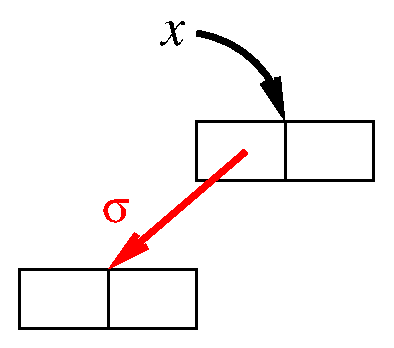
\epsfig{file=live-analysis1.eps, height=2cm}}
      \scalebox{.65}{
          \psset{unit=1mm}
          \psset{linewidth=.5mm}
          \begin{pspicture}(0,0)(90,0)
            %%%%%%%%%%%%%%%%%%%%%%%%%%%%%%%%%%%%%%%%%%%%%%%%%%%%%%%%%%%%%%%%
            \putnode{x}{origin}{13}{-10}{\TwoCells{x0}{x1}}
            \putnode{startx}{x}{0}{-3}{}
            \putnode{after0}{x}{-5}{-30}{}
            \putnode{result}{origin}{32}{10}{\TwoCells{resultx}{resulty}}
            \putnode{labx}{x}{-7}{10}{\large $(\CAR\ x)$\;{\red $\sigma$} }
            \putnode{labr}{result}{-12}{12}{\large $x$}
            
            \onslide<1>{\nccurve[nodesepB=-.2,nodesepA=.5,angleA=295,angleB=135]{->}{labr}{result}}
            \onslide<2>{\nccurve[nodesepB=-.2,nodesepA=.5,angleA=295,angleB=135,linecolor=red]{->}{labr}{result}}
            \nccurve[nodesepB=-.2,angleA=295,angleB=135]{->}{labx}{x}
            \onslide<1>{\nccurve[nodesepB=-.2,angleA=270,angleB=75]{*->}{resultx}{x} \bput(.5){\large \acar}}
            \onslide<2>{\nccurve[nodesepB=-.2,angleA=270,angleB=75,linecolor=red]{*->}{resultx}{x} \bput(.5){\large \acar}}
            \onslide<2>{\nccurve[nodesepB=-.2,angleA=270,angleB=75,
                linestyle=dashed,linecolor=red]{*->}{startx}{after0}
              \bput(.5){\large $\alpha$}}
          \end{pspicture}
      }
    \end{column}
    \begin{column}{0.65\textwidth}
      $\Lapp{{\red{(\CAR \;x)}}}{\sigma} = \{x.\epsilon, \; x.\acar\sigma\}$
    \end{column}
  \end{columns}
  \pause
  \bigskip
  \bigskip
  \bigskip
}
\only<3->{ 
  \begin{columns}[c]
    \begin{column}[T]{0.35\textwidth}
      %\centerline{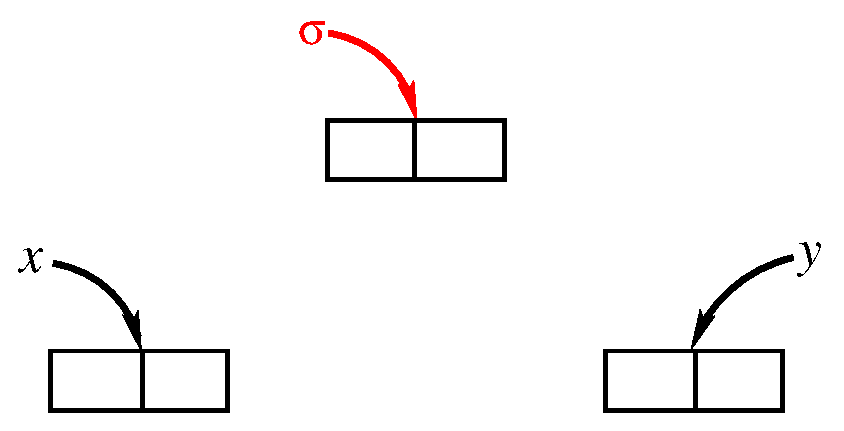
\epsfig{file=live-analysis2.eps, height=2.5cm}}
    \end{column}
    \begin{column}[T]{0.65\textwidth}
      \begin{minipage}{\textwidth}
        \begin{eqnarray*}
          \Lapp{{\red{(\CONS \;x \;y)}}}{\sigma} &=&  \{x.\alpha \mid \acar\alpha \in \sigma\} \; \cup\\
          & &  \{y.\beta \mid \acdr\beta \in \sigma\}
        \end{eqnarray*}
        
        \onslide<5->{
          \begin{itemize}
          \item 
            \bcar\ -- Removal of a leading \acar
            \\
            \bcdr\  -- Removal of a leading \acdr
            
          \end{itemize}
          \begin{eqnarray*}
            \Lapp{{\red{(\CONS \;x \;y)}}}{\sigma} &=&  x.\bcar\sigma \cup  y.\bcdr\sigma
        \end{eqnarray*}}
      \end{minipage}
    \end{column}
  \end{columns}

\raisebox{25mm}{\scalebox{.65}{
    \psset{unit=1mm}
    \psset{linewidth=.5mm}
    \begin{pspicture}(0,0)(90,0)
      %%%%%%%%%%%%%%%%%%%%%%%%%%%%%%%%%%%%%%%%%%%%%%%%%%%%%%%%%%%%%%%%
      \putnode{x}{origin}{-3}{40}{\TwoCells{x0}{x1}}
      \putnode{y}{x}{51}{0}{\TwoCells{y0}{y1}}
      \putnode{startx}{x}{0}{-3}{}
      \putnode{starty}{y}{0}{-3}{}
      \putnode{after0}{x}{-5}{-30}{}
      \putnode{after1}{y}{5}{-30}{}
      \putnode{result}{origin}{22}{60}{\TwoCells{resultx}{resulty}}
      \putnode{labx}{x}{-7}{10}{\large $x$}
      \putnode{laby}{y}{7}{10}{\large $y$}
      \putnode{labr}{result}{-12}{12}{\large $(\CONS\ x\ y)$\; {\red $\sigma$} }

      \nccurve[nodesepB=-.2,angleA=295,angleB=135]{->}{labr}{result}
      \nccurve[nodesepB=-.2,angleA=295,angleB=135]{->}{labx}{x}
      \nccurve[nodesepB=-.2,angleA=270,angleB=45]{->}{laby}{y}
      \nccurve[nodesepB=-.2,angleA=270,angleB=75]{*->}{resultx}{x}
      \onslide<4->{        \bput(.5){\large \acar}}
      \nccurve[nodesepB=-.2,angleA=270,angleB=105]{*->}{resulty}{y}
      \onslide<4->{        \aput(.5){\large \acdr}}
      \onslide<4->{\nccurve[nodesepB=-.2,angleA=270,angleB=75,
          linestyle=dashed]{*->}{startx}{after0}
        \bput(.5){\large $\alpha$}
	\nccurve[nodesepB=-.2,angleA=270,angleB=105,
          linestyle=dashed]{*->}{starty}{after1}
        \aput(.5){\large ${\mathbf \beta}$}}
    \end{pspicture}
}}}
\end{frame}

%%%%%%%%%%%%%%%%%%%%%%%%%%%%%%%%%%%%%%%%%%%%%%%%%%%%%%%
%%%%%%%%%%%%%%%%%%%%%%%%%%%%%%%%%%%%%%%%%%%%%%%%%%%%%%
%% \begin{frame}{Notational devices \bcar\ and \bcdr}
%% \small
%% Define \bcar\ and \bcdr\  as:
%% \begin{align*}
%% \bcar\sigma &= \{\alpha \mid \acar\alpha \in \sigma\}\\
%% \bcdr\sigma &= \{\alpha \mid \acdr\alpha \in \sigma\}
%% \end{align*}

%% Then we have:
%% \begin{eqnarray*}
%%     \Lapp{{\red{(\CONS \;x \;y)}}}{\sigma} &=&  x.\bcar\sigma \cup  y.\bcdr\sigma
%% \end{eqnarray*}

%% \bigskip

%% Bar removal relation $\hookrightarrow$ over sets of access paths:
%% \begin{eqnarray*}
%%   \sigma_1\bcar\sigma_2  \hookrightarrow 
%%   \sigma_1\sigma_2',\mbox{ where} \sigma_2'& =& \lbrace \alpha \mid
%%   \acar \alpha \in \sigma_2 \rbrace,
%%  \quad\mbox{and}\quad \\
%% \sigma_1\bcdr\sigma_2  \hookrightarrow 
%%   \sigma_1\sigma_2',\mbox{ where} \sigma_2'& =& \lbrace \alpha \mid
%%   \acdr \alpha \in \sigma_2 \rbrace  
%% \end{eqnarray*} 
%% \end{frame}

%% %% \bigskip
%% \hrule
%% \bigskip

%%   \begin{columns}[c]
%%   \begin{column}{0.33\textwidth}56
%%  \centerline{\epsfig{file=live-analysis3.eps, height=2cm}}
%%   \end{column}
%%  \begin{column}{0.67\textwidth}
%% \begin{minipage}{\textwidth}
%%     $\Lapp{{\red{(+ \;x \;y)}}}{\sigma} = \{x.\epsilon, \; y.\epsilon \}$
%% \end{minipage}
%%   \end{column}
%% \end{columns}




%%%%%%%%%%%%%%%%%%%%%%%%%%%%%%%%%%%%%%%%%%%%%%%%%%%%%%
%%%%%%%%%%%%%%%%%%%%%%%%%%%%%%%%%%%%%%%%%%%%%%%%%%%%%%

\begin{frame}{Liveness Analysis of Function Applications}
\onslide<1->{
  \begin{columns}[c]
    \begin{column}{0.4\textwidth}
      \onslide<1->{
        %\centerline{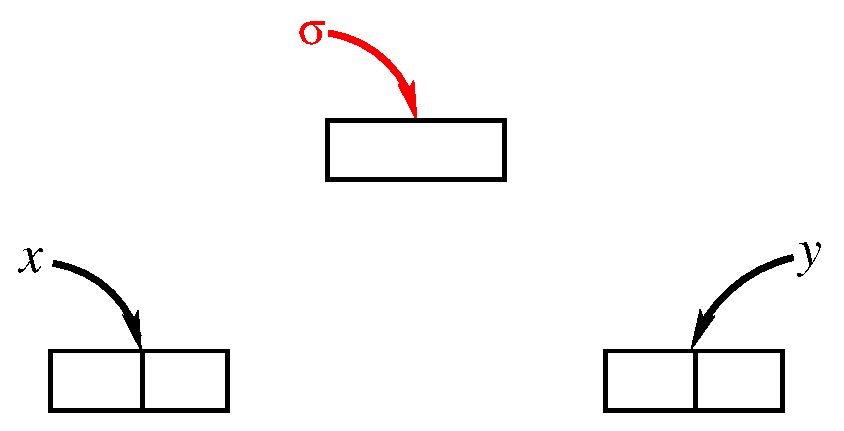
\epsfig{file=live-analysis4.eps, height=2.6cm}}
        \raisebox{-35mm}{\scalebox{.65}{
            \psset{unit=1mm}
            \psset{linewidth=.5mm}
            \begin{pspicture}(-10,0)(80,0)
              %%%%%%%%%%%%%%%%%%%%%%%%%%%%%%%%%%%%%%%%%%%%%%%%%%%%%%%%%%%%%%%%
              \putnode{x}{origin}{0}{30}{\TwoCells{x0}{x1}}
              \putnode{y}{x}{51}{0}{\TwoCells{y0}{y1}}
              \putnode{startx}{x}{0}{-3}{}
              \putnode{starty}{y}{0}{-3}{}
              \putnode{after0}{x}{-5}{-20}{}
              \putnode{after1}{y}{5}{-20}{}
              \putnode{result}{origin}{25}{50}{\OneCell{resultx}}
              \putnode{labx}{x}{-7}{10}{\large $x$}
              \putnode{laby}{y}{7}{10}{\large $y$}
              \putnode{labr}{result}{-12}{7}{\large $(f\ x\ y)$\; {\red $\sigma$} }
              
              \nccurve[nodesepB=-.2,angleA=295,angleB=135]{->}{labr}{result}
              \nccurve[nodesepB=-.2,nodesepA=.2,angleA=295,angleB=135]{->}{labx}{x}
              \nccurve[nodesepB=-.2,angleA=270,angleB=45]{->}{laby}{y}
              \onslide<2>{
                \nccurve[nodesepB=-.2,angleA=270,angleB=75,linestyle=dashed]{*->}{resultx}{x}
                \bput(.6){\large $\psi_x$}
                \nccurve[nodesepB=-.2,angleA=270,angleB=105,linestyle=dashed]{*->}{resultx}{y}
                \aput(.6){\large $\psi_y$}
              }
              \onslide<3->{
                \nccurve[nodesepB=-.2,angleA=270,angleB=75,linestyle=dashed]{*->}{resultx}{x}
                \bput(.6){\large \Lf{f}{1}{\alpha}}
                \nccurve[nodesepB=-.2,angleA=270,angleB=105,linestyle=dashed]{*->}{resultx}{y}
                \aput(.6){\large \Lf{f}{2}{\beta}}

              }
              \nccurve[nodesepB=-.2,angleA=270,angleB=105]{*->}{resulty}{y}
              \onslide<2->{\nccurve[nodesepB=-.2,angleA=270,angleB=75,
                  linestyle=dashed]{*->}{startx}{after0}
                \onslide<2>{\bput(.5){\large $\alpha$}}
	        \nccurve[nodesepB=-.2,angleA=270,angleB=105,
                  linestyle=dashed]{*->}{starty}{after1}
                \onslide<2>{\aput(.5){\large ${\mathbf \beta}$}}
              }
            \end{pspicture}
      }}}
    \end{column}
    \begin{column}{0.5\textwidth}
      \small
      \mbox{\onslide<1->{$\Lapp{{\red{(f \;x \;y)}}}{\sigma} =$}
        \onslide<2->{
          \alt<2>{$\{x.\overline{\psi_x}{\sigma},  \;  y.\overline{\psi_y}{\sigma}\}$}{$\{x.\Lf{f}{1}{\sigma},  \;  y.\Lf{f}{2}{\sigma}\}$}
        }}
    \end{column}
  \end{columns}
}
{
  \bigskip
  \begin{itemize}
    \onslide<3->{  \item We use \Lfonly$_{\mathit  f}$: context independent summary of
      the function $f$.}
    \onslide<4-> {\item To find \Lf{\mathit  f}{i}{\sigma}: 
      \begin{itemize}
      \item Assume a symbolic demand $\sigma$.
      \item Let $e_f$ be the body of $f$..  
      \item Set  \Lf{\mathit  f}{i}{\sigma} to \Lexp{e_f}{\sigma}($x_i$).
        \onslide<5->{
        \item How to handle recursive calls?         
          \onslide<6->{
            {\red Use the assumed  \Lfonly$_{\mathit  f}$~!!}
        }}
    \end{itemize}}
  \end{itemize}
}
\end{frame}

%%%%%%%%%%%%%%%%%%%%%%%%%%%%%%%%%%%%%%%%%%%%%%%%%%%%%%
%%%%%%%%%%%%%%%%%%%%%%%%%%%%%%%%%%%%%%%%%%%%%%%%%%%%%%

\begin{frame}[t]{Liveness analysis -- The big picture}

\setbeamercovered{transparent}
\small
\begin{columns}[c]
 \begin{column}[T]{0.5\textwidth}
\hspace*{-.3cm}\renewcommand{\arraystretch}{1}{
	  \begin{uprogram}
	  \UNL{1}\hspace*{-.2cm} $\pi_\mainpgm\!\!:\, $(\onslide<0>{\LET\  \pz\  $\leftarrow$ \ldots  \IN
	  \UNL{2}   \hspace*{.3cm}              (\LET\ \py\  $\leftarrow$  \ldots \IN}
          \UNL{3}   \hspace*{-.5cm}    $\pi_9\!\!:\, $\onslide<0>{(\LET\ \pw\  $\leftarrow$}  (\append\ \py\ \pz) \onslide<0>{\IN}
          \UNL{4}   \hspace*{-.8cm}  $\pi_{10}\!\!:\, $\onslide<0>{(\LET\ \pa\  $\leftarrow$  (\CDR\ \pw) \IN}
	  \UNL{5}   \hspace*{-1.1cm}  $\pi_{11}\!\!:\, $\onslide<0>{(\LET\ \pb\  $\leftarrow$ (\CAR\  \pa) \IN}
          \UNL{6}   \hspace*{-1.4cm} $\pi_{12}\!\!:\,$\onslide<0>{(\RETURN\ \pb))))))})
\end{uprogram}}
 \end{column}
 \begin{column}[T]{0.6\textwidth}
\hspace*{.4cm}  \renewcommand{\arraystretch}{1}{
  \begin{uprogram}
    \UNL{1}\hspace*{-.7cm} (\DEFINE\ (\append~\lista~\listb)

    \UNL{2}\hspace*{-1cm}  $\pi_1\!\!:\, $\onslide<0>{(\LET\ \xtest\ $\leftarrow $\ (\NULLQ~\lista) \IN}


    \UNL{3} \hspace*{-1.4cm}     $\pi_2\!\!:\, $\onslide<0>{(\SIF\ \xtest}

~$\pi_3\!\!:$\onslide<0>{(\RETURN\ \listb)} 
 
          \UNL{4}\hspace*{-1.8cm} \hspace*{.05cm}    
 $\pi_4\!\!:\, $\onslide<0>{(\LET\ \xtl\  $\leftarrow$\   (\CDR\ \lista) \IN}

	  \UNL{5}\hspace*{-2.1cm}  \hspace*{.05cm}    $\pi_5\!\!:\,$\onslide<0>{(\LET\ \xrec\  $\leftarrow$}\onslide<1->{  (\append\ \ \xtl\ \  \listb)}\onslide<0>{  \IN}


          \UNL{6}\hspace*{-2.4cm} \hspace*{.05cm}   $\pi_6\!\!:\, $\onslide<0>{(\LET\ \xhd\  $\leftarrow$  (\CAR\ \lista)  \IN}


          \UNL{7}\hspace*{-2.7cm}  \hspace*{.05cm}   $\pi_7\!\!:\,$\onslide<0>{(\LET\ \xans\  $\leftarrow$ (\CONS\ \ \xhd\ \ \xrec)  \IN 

          \UNL{8}\hspace*{-3.0cm} \hspace*{.05cm}}
$\pi_8\!\!:\, $ \onslide<0>{(\RETURN\ \xans)))))))}\onslide<1->{)}
\end{uprogram}}
 \end{column}
\end{columns}

\bigskip
\bigskip

\footnotesize
\begin{columns}[c]
 \begin{column}[T]{0.40\textwidth}
\scriptsize
\centerline{\bf Liveness environments:}

\bigskip

$\Lanv{1}{\lista} = \{\epsilon\} \cup  \acar\bcar\sigma\; \cup $\\
$\;\;\;\;\;\;\;\;\;\;\;\acdr\Lf{\append}{1}{\bcdr\sigma_{\append}}$\\
$\Lanv{1}{\listb} = \sigma \cup \Lf{\append}{2}{\bcdr\sigma_{\append}}$\\
%% \Lanv{5}{\lista} &= \{\epsilon\} \cup  \acar\bcar\sigma_{\append}\\
%% \Lanv{5}{\xtl} &= \Lf{\append}{1}{\bcdr\sigma_{\append}}\\
%% \Lanv{5}{\listb} &= \Lf{\append}{2}{\bcdr\sigma_{\append}}\\
\ldots\\
%% $\mbox{Program}\;  & \mbox{points in \mainpgm}\\ 
$\Lanv{9}{\py}  = $ \Lf{\append}{1}{\{\epsilon,
     \acdr\} \cup \acdr\acar\sigma_{\mathit{\!all}}} \\
%%   \Lanv{9}{\pz}  &= \Lf{\append}{2}{\{\epsilon,
%%     \acdr\} \cup \acdr\acar\sigma_{\mathit{\!all}}}\\$


 \end{column}
 \begin{column}[T]{0.30\textwidth}
\scriptsize
\centerline{\bf Demand summaries:}
%\begin{eqnarray*}
%\sigma_{\xmain} &=& \sigma_{all}\\
%\sigma_{\append} &=& \ldots
%\end{eqnarray*}
 \end{column}
 \begin{column}[T]{0.38\textwidth}
\scriptsize
\centerline{\bf Function summaries:}
\bigskip\onslide<2->{
$\Lf{\append}{1}{\sigma} = \{\epsilon\} \cup \acar\bcar\sigma ~
\cup$ \\ 
$ \;\;\;\;\;\;\;\;\;\;\;\;\;\;\;\;\;\;\;\;\;\;\acdr\Lf{\append}{1}{\bcdr\sigma}$\\
$\Lf{\append}{2}{\sigma} = \sigma \cup \Lf{\append}{2}{\bcdr\sigma}$
}
 \end{column}
\end{columns}
\end{frame}

%%%%%%%%%%%%%%%%%%%%%%%%%%%%%%%%%%%%%%%%%%%%%%%%%%%%%%
%%%%%%%%%%%%%%%%%%%%%%%%%%%%%%%%%%%%%%%%%%%%%%%%%%%%%%

\begin{frame}{Liveness analysis -- Demand Summary}

\setbeamercovered{transparent}
\small
\begin{columns}[c]
 \begin{column}[T]{0.5\textwidth}
\hspace*{-.3cm}\renewcommand{\arraystretch}{1}{
	  \begin{uprogram}
	  \UNL{1}\hspace*{-.2cm} $\pi_\mainpgm\!\!:\, $(\onslide<0>{\LET\  \pz\  $\leftarrow$ \ldots  \IN
	  \UNL{2}   \hspace*{.3cm}              (\LET\ \py\  $\leftarrow$  \ldots \IN}
          \UNL{3}   \hspace*{-.5cm}    $\pi_9\!\!:\, $\onslide<0>{(\LET\ \pw\  $\leftarrow$}  (\append\ \py\ \pz) \onslide<0>{\IN}
          \UNL{4}   \hspace*{-.8cm}  $\pi_{10}\!\!:\, $\onslide<0>{(\LET\ \pa\  $\leftarrow$  (\CDR\ \pw) \IN}
	  \UNL{5}   \hspace*{-1.1cm}  $\pi_{11}\!\!:\, $\onslide<0>{(\LET\ \pb\  $\leftarrow$ (\CAR\  \pa) \IN}
          \UNL{6}   \hspace*{-1.4cm} $\pi_{12}\!\!:\,$\onslide<0>{(\RETURN\ \pb))))))})
\end{uprogram}}
 \end{column}
 \begin{column}[T]{0.6\textwidth}
\hspace*{.4cm}  \renewcommand{\arraystretch}{1}{
  \begin{uprogram}
    \UNL{1}\hspace*{-.7cm} (\DEFINE\ (\append~\lista~\listb)

    \UNL{2}\hspace*{-1cm}  $\pi_1\!\!:\, $\onslide<0>{(\LET\ \xtest\ $\leftarrow $\ (\NULLQ~\lista) \IN}


    \UNL{3} \hspace*{-1.4cm}     $\pi_2\!\!:\, $\onslide<0>{(\SIF\ \xtest}

~$\pi_3\!\!:$\onslide<0>{(\RETURN\ \listb)} 
 
          \UNL{4}\hspace*{-1.8cm} \hspace*{.05cm}    
 $\pi_4\!\!:\, $\onslide<0>{(\LET\ \xtl\  $\leftarrow$\   (\CDR\ \lista) \IN}

	  \UNL{5}\hspace*{-2.1cm}  \hspace*{.05cm}
          $\pi_5\!\!:\,$\onslide<0>{(\LET\ \xrec\  $\leftarrow$} {  (\append\ \ \xtl\ \  \listb)}\onslide<0>{  \IN}


          \UNL{6}\hspace*{-2.4cm} \hspace*{.05cm}   $\pi_6\!\!:\, $\onslide<0>{(\LET\ \xhd\  $\leftarrow$  (\CAR\ \lista)  \IN}


          \UNL{7}\hspace*{-2.7cm}  \hspace*{.05cm}   $\pi_7\!\!:\,$\onslide<0>{(\LET\ \xans\  $\leftarrow$ (\CONS\ \ \xhd\ \ \xrec)  \IN 

          \UNL{8}\hspace*{-3.0cm} \hspace*{.05cm}}
$\pi_8\!\!:\, $ \onslide<0>{(\RETURN\ \xans)))))))}\onslide<1->{)}
\end{uprogram}}
 \end{column}
\end{columns}
\setbeamercovered{invisible}
      \raisebox{-25mm}{\scalebox{.85}{
	%%%%%%%%%%%%%%%%%%%%%Uday's stuff%%%%%%%%%%%%%%%%%%%%%%%%%
      \psset{unit=1mm}
      \psset{linewidth=.3mm}
      \begin{pspicture}(0,0)(180,30)
%\psgrid[xunit=1cm,yunit=1cm,gridwidth=.2pt,subgridwidth=.1pt,subgriddiv=5,subgridcolor=gray,gridcolor=blue](0,0)(18,10)
	%\psframe(0,0)(73,60)
	%%%%%%%%%%%%%%%%%%%%%%%%%%%%%%%%%%%%%%%%%%%%%%%%%%%%%%%%%%%%%%%%
	\onslide<1-5>{\putnode{o}{origin}{26}{72}{\large\red $\sigma_{\xmain} =
          \sigma{_{all}}$}}
	\onslide<2-5>{\putnode{call1}{origin}{38}{62}{\large\red $\sigma_1$} 
%$\{\epsilon, \; \acdr\} \cup    \acdr\acar\sigma_{all}$}
	\nccurve[nodesepB=-.2,angleA=270,angleB=135,linecolor=red]{->}{o}{call1}}
	\onslide<3-5>{\putnode{appendentry}{origin}{85}{72}{\large\red
          $\sigma_{\append} = \sigma_1 \cup \only<3-4>{\ldots} 
%\{\epsilon, \; \acdr\} \cup  \acdr\acar\sigma_{all} 
\only<5->{\sigma_2}$}
%{ \cup  \bcdr\sigma_{\append}}$}
	\nccurve[nodesepB=-.2,angleA=45,angleB=165,linecolor=red]{->}{call1}{appendentry}}
	\onslide<4-5>{\putnode{call2}{origin}{115}{52}{\large\red $\sigma_2$} 
%$\bcdr\sigma_{\append}$}
	\nccurve[nodesepB=-.2,angleA=270,angleB=135,linecolor=red]{->}{appendentry}{call2}}
	\onslide<5-5>{\nccurve[nodesepB=-.2,angleA=65,angleB=0,linecolor=red]{->}{call2}{appendentry}}

      \end{pspicture}}}

\vspace*{-2cm}
\footnotesize
\begin{columns}[c]
 \begin{column}[T]{0.40\textwidth}
\scriptsize
\centerline{\bf Liveness environments:}

\bigskip

$\Lanv{1}{\lista} = \{\epsilon\} \cup  \acar\bcar\sigma\; \cup $\\
$\;\;\;\;\;\;\;\;\;\;\;\acdr\Lf{\append}{1}{\bcdr\sigma_{\append}}$\\
$\Lanv{1}{\listb} = \sigma \cup \Lf{\append}{2}{\bcdr\sigma_{\append}}$\\
%% \Lanv{5}{\lista} &= \{\epsilon\} \cup  \acar\bcar\sigma_{\append}\\
%% \Lanv{5}{\xtl} &= \Lf{\append}{1}{\bcdr\sigma_{\append}}\\
%% \Lanv{5}{\listb} &= \Lf{\append}{2}{\bcdr\sigma_{\append}}\\
\ldots\\
%% $\mbox{Program}\;  & \mbox{points in \mainpgm}\\ 
$\Lanv{9}{\py}  = $ \Lf{\append}{1}{\{\epsilon,
     \acdr\} \cup \acdr\acar\sigma_{\mathit{\!all}}} \\
%%   \Lanv{9}{\pz}  &= \Lf{\append}{2}{\{\epsilon,
%%     \acdr\} \cup \acdr\acar\sigma_{\mathit{\!all}}}\\$


 \end{column}
 \begin{column}[T]{0.30\textwidth}
\scriptsize
\centerline{\bf Demand summaries:}
\onslide<6>{
\begin{align*}
&\sigma_{\xmain} = \sigma_{all}\\
&\sigma_{\append} = \{\epsilon, \; \acdr\} \cup
\acdr\acar\sigma_{all}\\
&\;\;\;\;\;  \cup  \bcdr\sigma_{\append}
\end{align*}
}
 \end{column}
 \begin{column}[T]{0.38\textwidth}
\scriptsize
\centerline{\bf Function summaries:}
\bigskip
$\Lf{\append}{1}{\sigma} = \{\epsilon\} \cup \acar\bcar\sigma ~
\cup$ \\ 
$ \;\;\;\;\;\;\;\;\;\;\;\;\;\;\;\;\;\;\;\;\;\;\acdr\Lf{\append}{1}{\bcdr\sigma}$\\
$\Lf{\append}{2}{\sigma} = \sigma \cup \Lf{\append}{2}{\bcdr\sigma}$
 \end{column}
\end{columns}
\end{frame}

%%%%%%%%%%%%%%%%%%%%%%%%%%%%%%%%%%%%%%%%%%%%%%%%%%%%%%
%%%%%%%%%%%%%%%%%%%%%%%%%%%%%%%%%%%%%%%%%%%%%%%%%%%%%%


%% \begin{frame}{Function Summaries \Lf{f}{i}{\sigma}}

%%   \begin{itemize}
%%   \item  \Lf{f}{i}{\sigma} answers the following question:

%% \bigskip

%% {\em  If the  demand  on the  result  of a  call  to $f$  is
%%   $\sigma$, then  what is the  liveness (alternately demand)
%%   of its $i^{th}$ argument?}


%% \bigskip
%% \bigskip

%% \item<2->    Analogy:   \Lf{\CONS}{1}{\sigma}   =    $\{\bcar\sigma\}$   and
%%   \Lf{\CONS}{2}{\sigma} = $\{\bcdr\sigma\}$.
%% \bigskip
%% \bigskip

%% \item<3-> To find \Lf{f}{i}{\sigma}: Let the body of $f$ be $e_f$. Find
%%   \Lexp{e_f}{\sigma}($x_i$)
%% \bigskip\bigskip


%%   \end{itemize}
%% \end{frame}

%%%%%%%%%%%%%%%%%%%%%%%%%%%%%%%%%%%%%%%%%%%%%%%%%%%%%%
%%%%%%%%%%%%%%%%%%%%%%%%%%%%%%%%%%%%%%%%%%%%%%%%%%%%%%

%% \begin{frame}[t]{An example}

%% \setbeamercovered{transparent}
%% \small

%% Start with a {\em symbolic demand {\red $\sigma$}}


%% \begin{center}
%% \begin{boxedminipage}{0.8\textwidth}
%%   \renewcommand{\arraystretch}{1}{
%%   \begin{uprogram}
%%     \UNL{1}\hspace*{-.7cm} (\DEFINE\ (\append~\lista~\listb)

%% \onslide<7->{ 	  
%%     \UNL{2}\hspace*{-1cm}  $\pi_1\!\!:\, $(\LET\ \xtest\ $\leftarrow $\ (\NULLQ~\lista) \IN
%%}
%% \onslide<6->{	  
%%     \UNL{3} \hspace*{-1cm}     $\pi_2\!\!:\, $(\SIF\ \xtest}
%% \onslide<1->{
%% ~$ \pi_3\!\!:$(\RETURN\ \listb)} 
 
%% \onslide<5->{
%%           \UNL{4}\hspace*{-1cm} \hspace*{.05cm}     $\pi_4\!\!:\, $(\LET\ \xtl\  $\leftarrow$\   (\CDR\ \lista) \IN}
%% \onslide<4->{
%% 	  \UNL{5}\hspace*{-1cm}  \hspace*{.05cm}    $\pi_5\!\!:\,$(\LET\ \xrec\  $\leftarrow$  (\append\ \ \xtl\ \  \listb) \IN}

%% \onslide<3->{ 
%%           \UNL{6}\hspace*{-1cm} \hspace*{.05cm}   $\pi_6\!\!:\, $ (\LET\ \xhd\  $\leftarrow$  (\CAR\ \lista)  \IN}

%% \onslide<2->{
%%           \UNL{7}\hspace*{-1cm}  \hspace*{.05cm}   $\pi_7\!\!:\,$ 
%%          (\LET\ \xans\  $\leftarrow$ (\CONS\ \ \xhd\ \ \xrec)  \IN 

%%           \UNL{8}\hspace*{-1cm} \hspace*{.05cm}}
                
%% \onslide<1->{$\pi_8\!\!:\, $  (\RETURN\ \xans)}\onslide<2->{)}\onslide<3->{)}\onslide<4->{)}\onslide<5->{)}\onslide<6->{)}\onslide<7->{)}\onslide<1->{)}
%% \end{uprogram}}
%% \end{boxedminipage}
%% \end{center}
%% \bigskip

%% \begin{columns}

%% \only<1>{
%% \begin{column}[T]{.5\textwidth}
%% \begin{align*}
%% \Lanv{8}{\xans} &= \sigma
%% \end{align*}
%% \end{column}
%%}

%% \only<2>{
%% \begin{column}[T]{.5\textwidth}
%% \begin{align*}
%% \Lanv{7}{\xhd} &= \bcar\sigma\\
%% \Lanv{7}{\xrec} &= \bcdr\sigma
%% \end{align*}
%% \end{column}
%%}

%% \only<3>{
%% \begin{column}[T]{.5\textwidth}
%% \begin{align*}
%%  \Lanv{6}{\lista} &= \{\epsilon\} \cup  \acar\bcar\sigma\\
%%  \Lanv{6}{\xrec} &= \bcdr\sigma
%% \end{align*}
%% \end{column}
%%}

%% \only<4>{
%% \begin{column}[T]{.5\textwidth}
%% \begin{align*}
%% \Lanv{5}{\lista} &= \{\epsilon\} \cup  \acar\bcar\sigma\\
%%  \Lanv{5}{\listb} &= \Lf{\append}{2}{\bcdr\sigma}\\
%%  \Lanv{5}{\xtl} &= \Lf{\append}{1}{\bcdr\sigma}
%% \end{align*}
%% \end{column}
%%}


%% \only<5>{
%% \begin{column}[T]{.5\textwidth}
%% \begin{align*}
%% \Lanv{4}{\lista} &= \{\epsilon\} \cup  \acar\bcar\sigma \cup \acdr\Lf{\append}{2}{\bcdr\sigma}\\
%%  \Lanv{4}{\listb} &= \Lf{\append}{2}{\bcdr\sigma}\\
%% % \Lanv{4}{\xtl} &= \Lf{\append}{1}{\bcdr\sigma}
%% \end{align*}
%% \end{column}
%%}

%% \only<6>{
%% \begin{column}[T]{.5\textwidth}
%% \begin{align*}
%% \Lanv{2}{\lista} &= \{\epsilon\} \cup  \acar\bcar\sigma \cup \acdr\Lf{\append}{1}{\bcdr\sigma}\\
%%   \Lanv{2}{\listb} &=  \sigma \cup \Lf{\append}{2}{\bcdr\sigma}\\
%% \Lanv{2}{\xtest} &= \{\epsilon\}
%% \end{align*}
%% \end{column}
%%}
%% \only<7>{
%% \begin{column}[T]{.5\textwidth}
%% \begin{align*}
%% \Lanv{2}{\lista} &= \{\epsilon\} \cup  \acar\bcar\sigma \cup \acdr\Lf{\append}{1}{\bcdr\sigma}\\
%%   \Lanv{2}{\listb} &=  \sigma \cup \Lf{\append}{2}{\bcdr\sigma}\\
%% \end{align*}
%% \end{column}
%%}

%% \onslide<1-5>{
%% \begin{column}[T]{.5\textwidth}
%% \begin{align*}
%% \Lanv{3}{\listb} &= \sigma
%% \end{align*}
%% \end{column}
%%}
%% \end{columns}

%% \end{frame}

%%\begin{align*}
%% \Lanv{7}{\xhd} &= \bcar\sigma\\
%% \Lanv{7}{\xrec} &= \bcdr\sigma
%% \end{align*}


%% \only<2>
%% {
%% \begin{center}
%% \begin{boxedminipage}{0.8\textwidth}
%% \renewcommand{\arraystretch}{1}{
%% 	  \begin{uprogram}
%% 	  \UNL{1}\hspace*{-.7cm} (\DEFINE\ (\append~\lista~\listb)
%% 	  \UNL{2}\hspace*{-1cm}  $\pi_1\!\!:\, $(\LET\ \xtest\ $\leftarrow $\ (\NULLQ~\lista) \IN
%% 	  \UNL{3} \hspace*{-1cm}     $\pi_2\!\!:\, $(\SIF\ \xtest~$\pi_3\!\!:$(\RETURN\ \listb)  
%%           \UNL{4}\hspace*{-1cm} \hspace*{.05cm}     $\pi_4\!\!:\, $(\LET\ \xtl\  $\leftarrow$\   (\CDR\ \lista) \IN
%% 	  \UNL{5}\hspace*{-1cm}  \hspace*{.05cm}    $\pi_5\!\!:\,${(\LET\ \xrec\  $\leftarrow$  (\append\ \ \xtl\ \  \listb) \IN}
%% 	  \UNL{6}\hspace*{-1cm} \hspace*{.05cm}   $\pi_6\!\!:\, $ (\LET\ \xhd\  $\leftarrow$  (\CAR\ \lista)  \IN
%% 	  \UNL{7}\hspace*{-1cm}  \hspace*{.05cm}   $\pi_7\!\!:\,$ {\red
%%           (\LET\ \xans\  $\leftarrow$ (\CONS\ \ \xhd\ \ \xrec)  \IN} 
%%           \UNL{8}\hspace*{-1cm} \hspace*{.05cm}    $\pi_8\!\!:\, $ {\red (\RETURN\ \xans)))})))))
%% 	\end{uprogram}}
%% \end{boxedminipage}
%% \end{center}
%% \bigskip
%% \begin{align*}
%% \Lanv{7}{\xhd} &= \bcar\sigma\\
%% \Lanv{7}{\xrec} &= \bcdr\sigma
%% \end{align*}
%%}

%% \only<3>
%% {
%% \begin{center}
%% \begin{boxedminipage}{0.8\textwidth}
%% \renewcommand{\arraystretch}{1}{
%% 	  \begin{uprogram}
%% 	  \UNL{1}\hspace*{-.7cm} (\DEFINE\ (\append~\lista~\listb)
%% 	  \UNL{2}\hspace*{-1cm}  $\pi_1\!\!:\, $(\LET\ \xtest\ $\leftarrow $\ (\NULLQ~\lista) \IN
%% 	  \UNL{3} \hspace*{-1cm}     $\pi_2\!\!:\, $(\SIF\ \xtest~$\pi_3\!\!:$(\RETURN\ \listb)  
%%           \UNL{4}\hspace*{-1cm} \hspace*{.05cm}     $\pi_4\!\!:\, $(\LET\ \xtl\  $\leftarrow$\   (\CDR\ \lista) \IN
%% 	  \UNL{5}\hspace*{-1cm}  \hspace*{.05cm}    $\pi_5\!\!:\,${(\LET\ \xrec\  $\leftarrow$  (\append\ \ \xtl\ \  \listb) \IN}
%% 	  \UNL{6}\hspace*{-1cm} \hspace*{.05cm}   $\pi_6\!\!:\, ${\red (\LET\ \xhd\  $\leftarrow$  (\CAR\ \lista)  \IN}
%% 	  \UNL{7}\hspace*{-1cm}  \hspace*{.05cm}   $\pi_7\!\!:\,$ {\red
%%           (\LET\ \xans\  $\leftarrow$ (\CONS\ \ \xhd\ \ \xrec)  \IN} 
%%           \UNL{8}\hspace*{-1cm} \hspace*{.05cm}    $\pi_8\!\!:\, $ {\red (\RETURN\ \xans)))})))))
%% 	\end{uprogram}}
%% \end{boxedminipage}
%% \end{center}
%% \bigskip
%% \begin{align*}
%% \Lanv{6}{\lista} &= \{\epsilon\} \cup  \acar\bcar\sigma\\
%% \Lanv{6}{\xrec} &= \bcdr\sigma
%% \end{align*}
%%}

%% \only<4>
%% {
%% \begin{center}
%% \begin{boxedminipage}{0.8\textwidth}
%% \renewcommand{\arraystretch}{1}{
%% 	  \begin{uprogram}
%% 	  \UNL{1}\hspace*{-.7cm} (\DEFINE\ (\append~\lista~\listb)
%% 	  \UNL{2}\hspace*{-1cm}  $\pi_1\!\!:\, $(\LET\ \xtest\ $\leftarrow $\ (\NULLQ~\lista) \IN
%% 	  \UNL{3} \hspace*{-1cm}     $\pi_2\!\!:\, $(\SIF\ \xtest~$\pi_3\!\!:$(\RETURN\ \listb)  
%%           \UNL{4}\hspace*{-1cm} \hspace*{.05cm}     $\pi_4\!\!:\, $(\LET\ \xtl\  $\leftarrow$\   (\CDR\ \lista) \IN
%% 	  \UNL{5}\hspace*{-1cm}  \hspace*{.05cm}    $\pi_5\!\!:\,${\red (\LET\ \xrec\  $\leftarrow$  (\append\ \ \xtl\ \  \listb) \IN}
%% 	  \UNL{6}\hspace*{-1cm} \hspace*{.05cm}   $\pi_6\!\!:\, ${\red (\LET\ \xhd\  $\leftarrow$  (\CAR\ \lista)  \IN}
%% 	  \UNL{7}\hspace*{-1cm}  \hspace*{.05cm}   $\pi_7\!\!:\,$ {\red
%%           (\LET\ \xans\  $\leftarrow$ (\CONS\ \ \xhd\ \ \xrec)  \IN} 
%%           \UNL{8}\hspace*{-1cm} \hspace*{.05cm}    $\pi_8\!\!:\, $ {\red (\RETURN\ \xans))))}))))
%% 	\end{uprogram}}
%% \end{boxedminipage}
%% \end{center}
%% \begin{align*}
%% \Lanv{5}{\lista} &= \{\epsilon\} \cup  \acar\bcar\sigma\\
%% \Lanv{5}{\xtl} &= \Lf{\append}{1}{\bcdr\sigma}\\
%% \Lanv{5}{\listb} &= \Lf{\append}{2}{\bcdr\sigma}
%% \end{align*}

%}

%% \only<5->
%% {
%% \begin{center}
%% \begin{boxedminipage}{0.8\textwidth}
%% \renewcommand{\arraystretch}{1}{
%% 	  \begin{uprogram}
%% 	  \UNL{1}\hspace*{-.7cm} (\DEFINE\ (\append~\lista~\listb)
%% 	  \UNL{2}\hspace*{-1cm}  $\pi_1\!\!:\, ${\red (\LET\ \xtest\ $\leftarrow $\ (\NULLQ~\lista) \IN}
%% 	  \UNL{3} \hspace*{-1cm}     $\pi_2\!\!:\, ${\red (\SIF\ \xtest~$\pi_3\!\!:$(\RETURN\ \listb)} 
%%           \UNL{4}\hspace*{-1cm} \hspace*{.05cm}     $\pi_4\!\!:\, ${\red (\LET\ \xtl\  $\leftarrow$\   (\CDR\ \lista) \IN}
%% 	  \UNL{5}\hspace*{-1cm}  \hspace*{.05cm}    $\pi_5\!\!:\,${\red (\LET\ \xrec\  $\leftarrow$  (\append\ \ \xtl\ \  \listb) \IN}
%% 	  \UNL{6}\hspace*{-1cm} \hspace*{.05cm}   $\pi_6\!\!:\, ${\red (\LET\ \xhd\  $\leftarrow$  (\CAR\ \lista)  \IN}
%% 	  \UNL{7}\hspace*{-1cm}  \hspace*{.05cm}   $\pi_7\!\!:\,$ {\red
%%           (\LET\ \xans\  $\leftarrow$ (\CONS\ \ \xhd\ \ \xrec)  \IN} 
%%           \UNL{8}\hspace*{-1cm} \hspace*{.05cm}    $\pi_8\!\!:\, $ {\red (\RETURN\ \xans)))))))})
%% 	\end{uprogram}}
%% \end{boxedminipage}
%% \end{center}
%% \bigskip
%%}
%% \only<5>
%% {
%% \begin{align*}
%% \Lanv{1}{\lista} &= \{\epsilon\} \cup  \acar\bcar\sigma \cup \acdr\Lf{\append}{1}{\bcdr\sigma}\\
%% \Lanv{1}{\listb} &= \{\epsilon\} \cup \Lf{\append}{2}{\bcdr\sigma}
%% \end{align*}
%%}
%% \only<6>
%% {

%% \Lf{\append}{i}{\sigma} gives the liveness of the $i^{th}$ argument, when the demand on a call to \append\  is $\sigma$.
%%}
%% \only<7->
%% {
%% \begin{columns}[c]
%%   \begin{column}{0.4\textwidth}
%% \only<7->
%%     {    
%% \begin{align*}
%%       \Lanv{1}{\lista} &= \{\epsilon\} \cup \acar\bcar\sigma \cup \acdr\Lf{\append}{1}{\bcdr\sigma}\\
%%       \Lanv{1}{\listb} &= \sigma \cup \Lf{\append}{2}{\bcdr\sigma}
%%     \end{align*}
%%}
%%   \end{column}
%%   \begin{column}{0.60\textwidth}
%% \only<8->
%%     {\blue
%%     \begin{align*}
%%       \Lf{\append}{1}{\sigma} &= \{\epsilon\} \cup \acar\bcar\sigma
%%       \cup \acdr\Lf{\append}{1}{\bcdr\sigma}\\
%%       \Lf{\append}{2}{\sigma} &= \sigma \cup \Lf{\append}{2}{\bcdr\sigma}
%%     \end{align*}
%%}
%% \end{column}
%% \end{columns}


%%%%%%%%%%%%%%%%%%%%%%%%%%%%%%%%%%%%%%%%%%%%%%%%%%%%%%
%%%%%%%%%%%%%%%%%%%%%%%%%%%%%%%%%%%%%%%%%%%%%%%%%%%%%%

%% \begin{frame}{The demand on \append}
%%   \small
%% \begin{columns}[c]
%%   \begin{column}{0.5\textwidth}
%% \renewcommand{\arraystretch}{1}{
%% 	  \begin{uprogram}
%% 	  \UNL{1}\hspace*{-.7cm} (\DEFINE\ (\append~\lista~\listb)
%% 	  \UNL{2}\hspace*{-.8cm}  $\pi_1\!\!:\, ${ (\LET\ \xtest\ $\leftarrow $\ (\NULLQ~\lista) \IN}
%% 	  \UNL{3} \hspace*{-.8cm}     $\pi_2\!\!:\, ${ (\SIF\ \xtest~$\pi_3\!\!:$(\RETURN\ \listb)} 
%%           \UNL{4}\hspace*{-.8cm} \hspace*{.05cm}     $\pi_4\!\!:\, ${(\LET\ \xtl\  $\leftarrow$\   (\CDR\ \lista) \IN}
%% 	  \UNL{5}\hspace*{-.8cm}  \hspace*{.05cm}    $\pi_5\!\!:\,${ (\LET\ \xrec\  $\leftarrow$ {\red$\pi_{call_2}\!\!:\, $  (\append\ \ \xtl\ \  \listb)} \IN}
%% 	  \UNL{6}\hspace*{-.8cm} \hspace*{.05cm}   $\pi_6\!\!:\, ${ (\LET\ \xhd\  $\leftarrow$  (\CAR\ \lista)  \IN}
%% 	  \UNL{7}\hspace*{-.8cm}  \hspace*{.05cm}   $\pi_7\!\!:\,$  (\LET\ \xans\  $\leftarrow$ (\CONS\ \ \xhd\ \ \xrec)  \IN  
%%           \UNL{8}\hspace*{-.8cm} \hspace*{.05cm}    $\pi_8\!\!:\, $ { (\RETURN\ \xans))))}))))
%% 	\end{uprogram}}
%% \renewcommand{\arraystretch}{1}{
%% 	  \begin{uprogram}
%% 	  \UNL{1}\hspace*{-.7cm} $\pi_\mainpgm\!\!:\, $(\LET\  \pz\  $\leftarrow$ \ldots  \IN
%% 	  \UNL{2}   \hspace*{0.2cm}              (\LET\ \py\  $\leftarrow$  \ldots \IN 
%%           \UNL{3}   \hspace*{0.2cm}    $\pi_9\!\!:\, $(\LET\ \pw\   $\leftarrow$ {\red$\pi_{call_1}\!\!:\, $  (\append\ \py\ \pz)} \IN
%%           \UNL{4}   \hspace*{0.2cm}  $\pi_{10}\!\!:\, $  (\LET\ \pa\  $\leftarrow$  (\CDR\ \pw) \IN
%% 	  \UNL{5}   \hspace*{0.2cm}  $\pi_{11}\!\!:\, $
%%           (\LET\ \pb\  $\leftarrow$ (\CAR\  \pa) \IN
%%           \UNL{6}\hspace*{0.2cm} $\pi_{12}\!\!:\,${ (\RETURN\ \pb)}))))))
%% \end{uprogram}}
%%   \end{column}

%%   \begin{column}{0.5\textwidth}
%% \vspace*{-5.5cm}
%%     \begin{itemize}
%%     \item \only<1> {The demand on \mainpgm\  is $\sigma_{all} = (0+1)^*$.}
%% \only<2> {$\sigma_{call_1} = \{\epsilon, \; \acdr\} \cup    \acdr\acar\sigma_{all}$\\
%%           $\sigma_{call_2} = \bcdr\sigma_{\append} $}
%% \only<3> {$\sigma_{\append} = \{\epsilon, \; \acdr\} \cup
%%   \bcdr\sigma_{\append}\cup  \acdr\acar\sigma_{all}$}
%%     \end{itemize}
%%   \end{column}
%%   \end{columns}

%%\end{frame}

%%%%%%%%%%%%%%%%%%%%%%%%%%%%%%%%%%%%%%%%%%%%%%%%%%%%%%
%%%%%%%%%%%%%%%%%%%%%%%%%%%%%%%%%%%%%%%%%%%%%%%%%%%%%%
%% \begin{frame}[t]{Summary of Analysis Results}
%% \setbeamercovered{transparent}
%% \small 
%% For each function $f$, we have:
%% \begin{itemize}
%% \item<1-> Equations representing the  summary demand $\sigma_f$ on the
%%   body of $f$.
%% \item<2-> Equations representing the liveness at different program points $f$.
%% \item<3-> The summary function \Lfonly$_f$\ 
%% \end{itemize}
%% \scriptsize
%% \onslide<4>{
%% {\gray 
%% \hspace*{-1cm}\noindent\rule{12.8cm}{0.2pt}}}
%% \vspace*{-.7cm}
%% \begin{columns}[c]
%%   \begin{column}[T]{0.33\textwidth}
%% \onslide<1,4>
%% {
%%     \begin{align*}
%% \sigma_{\append} &= \{\epsilon, \; \acdr\} \cup
%%   \bcdr\sigma_{\append}\\
%% & \;\;\;\;\;\cup  \acdr\acar\sigma_{all}
%%     \end{align*}
%%}
%%   \end{column}
%% \onslide<4>{{\gray \vrule{}}}
%%   \begin{column}[T]{0.33\textwidth}
%% \onslide<2,4>
%% {
%% \begin{align*}
%% \mbox{Program}\; & \mbox{points in \append}\\ 
%% \Lanv{1}{\lista} &= \{\epsilon\} \cup  \acar\bcar\sigma\; \cup \\
%% &\;\;\;\;\;\acdr\Lf{\append}{1}{\bcdr\sigma_{\append}}\\
%% \Lanv{1}{\listb} &= \sigma \cup \Lf{\append}{2}{\bcdr\sigma_{\append}}\\
%% %% \Lanv{5}{\lista} &= \{\epsilon\} \cup  \acar\bcar\sigma_{\append}\\
%% %% \Lanv{5}{\xtl} &= \Lf{\append}{1}{\bcdr\sigma_{\append}}\\
%% %% \Lanv{5}{\listb} &= \Lf{\append}{2}{\bcdr\sigma_{\append}}\\
%% \ldots\\
%% \mbox{Program}\;  & \mbox{points in \mainpgm}\\ 
%%   \Lanv{9}{\py}  &= \Lf{\append}{1}{\{\epsilon,
%%     \acdr\} \cup \acdr\acar\sigma_{\mathit{\!all}}} \\
%%   \Lanv{9}{\pz}  &= \Lf{\append}{2}{\{\epsilon,
%%     \acdr\} \cup \acdr\acar\sigma_{\mathit{\!all}}}\\
%% \dots
%% \end{align*}
%%}
%%   \end{column}
%% \onslide<4>{{\gray \vrule{}}}
%% \begin{column}[T]{0.33\textwidth}
%% \onslide<3->
%%       {    
%% \begin{align*}
%%   \Lf{\append}{1}{\sigma} &= \{\epsilon\} \cup \acar\bcar\sigma\cup\\
%%   &\;\;\;\;\;  \acdr\Lf{\append}{1}{\bcdr\sigma}\\
%%   \Lf{\append}{2}{\sigma} &= \sigma \cup \Lf{\append}{2}{\bcdr\sigma}
%%       \end{align*}}
%%   \end{column}
%% \end{columns}
%% \onslide<4>{\gray 
%% \hspace*{-1cm}\noindent\rule{12.8cm}{0.4pt}}
%% \end{frame}
%%%%%%%%%%%%%%%%%%%%%%%%%%%%%%%%%%%%%%%%%%%%%%%%%%%%%%
%%%%%%%%%%%%%%%%%%%%%%%%%%%%%%%%%%%%%%%%%%%%%%%%%%%%%%
\begin{frame}{Obtaining a closed form solution for  \Lfonly}
  \begin{itemize}
%  \item<1-3> Unlike $\sigma_{\append}$ and $\Lanv{i}{x}$, the
%    solution of \Lfonly\ is a function.
%  \item<2-3>       Analogy:        The        solution        of
%    $\mathit{ay}''+\mathit{by}'+\mathit{c} = 0$ the solution
%    is a function.
  \item<1-> Function summaries will always have the form:
    \begin{align*}
      \Lf{f}{i}{\sigma} = \Uf{f}{i} \cup \Df{f}{i}\sigma
    \end{align*}
\item<2-> Consider the  equation for $\Lfonly^{1}_{\append}$
    \begin{align*}
{\red\Lf{\append}{1}{\sigma}} = \{\epsilon\} \cup \acar\bcar\sigma ~
\cup \acdr{\red \Lf{\append}{1}{\bcdr\sigma}}
    \end{align*}
\item<3->Substitute the assumed  form in the equation:
    \begin{align*}
        {\red\Uf{\append}{1}   \cup    \Df{\append}{1}\sigma}
        &= \{\epsilon\}\;  \cup\;
      \acar\bcar\sigma\cup  
      \acdr({\red\Uf{\append}{1} \cup
      \Df{\append}{1}\bcdr\sigma})
    \end{align*}
\item<3-> Equating the terms without and with $\sigma$, we get:  
    \begin{align*}
        \Uf{\append}{1} &= \{\epsilon\}\;  \cup\;
      \acdr\Uf{\append}{1}\\
  \Df{\append}{1} &= \acar\bcar\cup\acdr \Df{\append}{1}\bcdr
    \end{align*}
  \end{itemize}
\end{frame}
%%%%%%%%%%%%%%%%%%%%%%%%%%%%%%%%%%%%%%%%%%%%%%%%%%%%%%
%%%%%%%%%%%%%%%%%%%%%%%%%%%%%%%%%%%%%%%%%%%%%%%%%%%%%%

\begin{frame}[t]{Summary of Analysis Results}
%% \small 
%% For each function $f$, we have:
%% \begin{itemize}
%% \item<1> Equations representing the  summary demand $\sigma_f$ on the
%%   body of $f$.
%% \item<1> Equations representing the liveness at different
%%   program points $f$ {\red with \Lfonly\  substituted out.}
%% \item<1> {\red Equations for  \Ufonly$_f$ and \Dfonly$_f$}
%% \end{itemize}
\scriptsize
%\onslide<1>{
%% {\gray 
%% \hspace*{-1cm}\noindent\rule{12.8cm}{0.2pt}}

\begin{columns}[c]
  \begin{column}[T]{0.33\textwidth}
\vspace*{1.5cm}
\centerline{\bf Liveness at program points:}
  \begin{align*}
    \Lanv{1}{\lista} &= \{\epsilon\} \cup  \acar\bcar\sigma\; \cup \\
    &\;\;\;\;\;\acdr({\red \Uf{\append}{1} \cup \Df{\append}{1}\bcdr\sigma_{\append}})\\
    \Lanv{1}{\listb} &= \{\epsilon\} \cup {\red \Uf{\append}{2}}\\
    &\;\;\;\;\;{\red  \cup\  \Df{\append}{2}\bcdr\sigma_{\append}}\\
    \Lanv{5}{\lista} &= \{\epsilon\} \cup  \acar\bcar\sigma_{\append}\\
    \Lanv{5}{\xtl} &= {\red \Uf{\append}{1} \cup \Df{\append}{1}\bcdr\sigma_{\append}}\\
    \Lanv{5}{\listb} &= {\red \Uf{\append}{2} \cup \Df{\append}{2}\bcdr\sigma_{\append}}\\
    \ldots\\
    %\Lanv{8}{\xans} &= \sigma_{\append}
  \end{align*}
  \end{column}
%\onslide<4>{{\gray \vrule{}}}
\begin{column}[T]{0.33\textwidth}
\vspace*{1.5cm}
\centerline{\bf Demand summaries:}
     \begin{align*}
       \sigma_{\append} &= \{\epsilon, \; \acdr\} \cup
       \bcdr\sigma_{\append}\\
       & \;\;\;\;\;\cup  \acdr\acar\sigma_{all}
     \end{align*}
\end{column}
\begin{column}[T]{0.33\textwidth}
\vspace*{1.5cm}
\centerline{\bf Function summaries:}
{\red
\begin{align*}
        \Uf{\append}{1} &= \{\epsilon\}\;  \cup\;
      \acdr\Uf{\append}{1}\\
  \Df{\append}{1} &= \acar\bcar\cup\acdr \Df{\append}{1}\bcdr\\
  \Uf{\append}{2} &= \Uf{\append}{2}\\
  \Df{\append}{2} &= \{\epsilon\} \cup \Df{\append}{2}\bcar
  \end{align*}}
  \end{column}
\end{columns}
\end{frame}
%%%%%%%%%%%%%%%%%%%%%%%%%%%%%%%%%%%%%%%%%%%%%%%%%%%%%%
%%%%%%%%%%%%%%%%%%%%%%%%%%%%%%%%%%%%%%%%%%%%%%%%%%%%%%

\begin{frame}{Solution of the equations}

  View the equations as grammar rules:
\begin{eqnarray*}
    \Lanv{1}{\lista} &\rightarrow& \epsilon \mid  \acar\bcar\sigma\; \mid 
    \acdr({\red \Uf{\append}{1} \mid \Df{\append}{1}\bcdr\sigma_{\append}})\\
  \Uf{\append}{1}    &\rightarrow&    \epsilon   \mid
   \acdr{\Uf{\append}{1}}\\         
   \Df{\append}{1}
   &\rightarrow&               \acar\bcar               \mid
   \acdr\Df{\append}{1}\bcdr\\
 \end{eqnarray*}
The  solution of \Lanv{1}{\lista} is the   language  $\mathscr{L}(\Lanv{1}{\lista})$ generated    by    it.
\end{frame}

%%%%%%%%%%%%%%%%%%%%%%%%%%%%%%%%%%%%%%%%%%%%%%%%%%%%%%

%%%%%%%%%%%%%%%%%%%%%%%%%%%%%%%%%%%%%%%%%%%%%%%%%%%%%%
\begin{frame}{Working of Liveness-based GC (Mark phase)}
  \begin{itemize}
  \item GC invoked at a program point $\pi$
  \item GC traverses a path $\alpha$ starting from a root variable $x$.
  \item GC consults $\Lanv{}{x}$: 
    \begin{itemize}
    \item Does $\alpha \in \mathscr{L}(\Lanv{\pi}{x})$ ?
    \item If yes, then mark the current cell
    \end{itemize}
  \item  Note  that  $\alpha$  is a  {\em  forward}-only  access  path
    \begin{itemize}
    \item consisting  only of  edges \acar\  and \acdr,  but not  \bcar\ or
      \bcdr
    \item But $\mathscr{L}(\Lanv{\pi}{x})$ has access paths marked with \bcar/\bcdr\ for \acar/\acdr\  removal
  arising from the \CONS\  rule.
    \end{itemize}
  \end{itemize}
\end{frame}
%%%%%%%%%%%%%%%%%%%%%%%%%%%%%%%%%%%%%%%%%%%%%%%%%%%%%%
\begin{frame}{\bcar/\bcdr\ handling}

\begin{itemize}
\item \acar\   removal from a set of access paths:
\begin{align*}
\alpha_1\bcar\acar\alpha_2 &\hookrightarrow
  \alpha_1\alpha_2\\
\alpha_1\bcar \acdr\alpha_2 &\hookrightarrow
  \mbox{ drop $\alpha_1\bcar \acdr \alpha_2$ from the set}
\end{align*}
\item \acdr\   removal from a set of access paths:
\begin{align*}
\alpha_1\bcdr\acdr\alpha_2 &\hookrightarrow
  \alpha_1\alpha_2\\
\alpha_1\bcdr \acar\alpha_2 &\hookrightarrow
  \mbox{ drop $\alpha_1\bcdr \acar \alpha_2$ from the set}
\end{align*}
\end{itemize}

\end{frame}
%%%%%%%%%%%%%%%%%%%%%%%%%%%%%%%%%%%%%%%%%%%%%%%%%%%%%%
\begin{frame}{GC decision problem}

%% Let $x.\alpha$ be  a forward  access path.     Let
%% $\mathscr{L}(\Lanv{}{x})  \stackrel{*}\hookrightarrow  \sigma$,  where
%% $\sigma$ consists of forward access  paths only. Then does $\alpha \in
%% \sigma$?
%% \bigskip \pause
\begin{itemize}
\item Deciding the
  membership in  a CFG augmented  with a
  fixed set of unrestricted productions.
  \begin{align*}
    \bcar\acar    \rightarrow    \epsilon\\
    \bcdr\acdr    \rightarrow   \epsilon\\
  \end{align*}
\item The problem shown to be undecidable\footnote{ Prasanna, Sanyal, and Karkare. {\em Liveness-Based Garbage Collection for Lazy Languages}, submitted.}.
  \begin{itemize}
  \item Reduction from Halting problem.
  \end{itemize}
\end{itemize}
\end{frame}
%%%%%%%%%%%%%%%%%%%%%%%%%%%%%%%%%%%%%%%%%%%%%%%%%%%%%%
\begin{frame}{Practical \bcar/\bcdr\  simplification}

\begin{itemize}
\item The simplification is possible to do on a finite state automaton.
\item Over-approximate the CFG by an automaton
  (Mohri-Nederhoff transformation).
\item Perform \acar/\acdr\ removal on the automaton.
\end{itemize}

\end{frame}
%%%%%%%%%%%%%%%%%%%%%%%%%%%%%%%%%%%%%%%%%%%%%%%%%%%%%%
\begin{frame}{Example}
  \scriptsize
  \begin{columns}[c]
    \begin{column}[T]{.5\textwidth}
      {Grammar for \Lanv{9}{\py}}
      \begin{eqnarray*}
        \Lanv{9}{y}  &\rightarrow&  {\Uf{\append}{1}} \mid  {\Df
          {\append}{1}}        (\epsilon         \mid        \acdr   \mid
        \acdr\acar {\sigma_{\mathit{\!all}}})\\
        \Uf{\append}{1}    &\rightarrow&    \epsilon   \mid
        \acdr{\Uf{\append}{1}}\\         
        \Df{\append}{1}
        &\rightarrow&               \acar\bcar               \mid
        \acdr\Df{\append}{1}\bcdr\\
        \sigma_{\mathit{\!all}} &\rightarrow & \epsilon \mid \acar
        \sigma_{\mathit{\!all}} \mid \acdr
        \sigma_{\mathit{\!all}}
      \end{eqnarray*}
    \end{column}
    \begin{column}[T]{.5\textwidth}
      After Mohri-Nederhoff transformation
      \begin{eqnarray*}
        \Lanv{9}{y}  &\rightarrow&  {\Uf{\append}{1}} \mid  {\Df
          {\append}{1}}        (\epsilon         \mid        \acdr   \mid
        \acdr\acar {\sigma_{\mathit{\!all}}})\\
        \Uf{\append}{1}    &\rightarrow&    \epsilon   \mid
        \acdr{\Uf{\append}{1}}\\   
        \Df{\append}{1}
        &\rightarrow&               \acar\bcar \Dfbar{\append}{1}  \mid
        \acdr\Df{\append}{1} \\ 
                {\Dfbar{\append}{1}}  &\rightarrow&   \bcdr{\Dfbar{\append}{1}}
                \mid \epsilon \\
                \sigma_{\mathit{\!all}} &\rightarrow & \epsilon \mid \acar
                \sigma_{\mathit{\!all}} \mid \acdr
                \sigma_{\mathit{\!all}}
      \end{eqnarray*}
    \end{column}
  \end{columns}
\end{frame}
%%%%%%%%%%%%%%%%%%%%%%%%%%%%%%%%%%%%%%%%%%%%%%%%%%%%%%
\begin{frame}{Automaton for \Lanv{9}{y}}
\newcommand{\nfaD}{%
  \scalebox{.99}{
    \psset{unit=1mm,nodesep=0mm,labelsep=0.5mm}
    \begin{pspicture}(3,-1)(28,9)%\psgrid
      \putnode{t0}{origin}{-4}{15}{\Lf{\plength}{1}{\sigma}} 
      \putnode{t1}{t0}{20}{0}{\pscirclebox{\mbox{$q_0$}}}
      \hspace{5mm} 
      \putnode{t2}{t1}{15}{0}{\pscirclebox[doubleline=true]{\mbox{$q_1$}}} 
      \psset{arrows=->} \ncline{t0}{t1} 
      \ncline{t1}{t2} 
      \putnode{l0}{t1}{7}{2}{\clazy} 
      \nccurve[angleA=45, angleB=135, ncurv=2, nodesep=-1]{t1}{t1} 
      \putnode{l1}{t1}{0}{6}{\acdr, \clazy} 
      \nccurve[angleA=45,
        angleB=135, ncurv=1.5, nodesep=-1]{t2}{t2} 
      \putnode{l2}{t2}{0}{7}{\clazy}
    \end{pspicture}
}}

\newcommand{\zcarliveness}{%
  \scalebox{.99}{
    \psset{unit=1mm,nodesep=0mm,labelsep=0.5mm}
    \begin{pspicture}(3,-1)(28,9)%\psgrid
      \putnode{t0}{origin}{2}{1}{\mbox{zcar}} 
      \putnode{t1}{t0}{18}{0}{\pscirclebox{\mbox{$q_0$}}}
      \hspace{5mm} 
      \putnode{t2}{t1}{15}{5}{\pscirclebox{\mbox{$q_1$}}} 
      \putnode{t3}{t2}{15}{0}{\pscirclebox[doubleline=true]{\mbox{$q_2$}}} 
      \psset{arrows=->} \ncline{t0}{t1} 
      \ncline{t1}{t2} 
      \ncline{t2}{t3} 
      \putnode{l0}{t1}{7}{5}{\bcar} 
      \putnode{l1}{t2}{7}{2}{\acar}
      \putnode{t4}{t1}{15}{-5}{\pscirclebox[doubleline=true]{\mbox{$q_3$}}}
      \ncline{t1}{t4}
      \putnode{l2}{t1}{7}{0}{\bcar} 
      \nccurve[angleA=-45, angleB=-135, ncurv=1.5, nodesep=-1]{t4}{t4} 
      \putnode{l3}{t4}{0}{-8}{\acdr} 
    \end{pspicture}
}}

\newcommand{\zcarlivenesssimpl}{%
  \scalebox{.99}{
    \psset{unit=1mm,nodesep=0mm,labelsep=0.5mm}
    \begin{pspicture}(3,-1)(28,9)%\psgrid
      \putnode{t0}{origin}{2}{1}{\mbox{zcar}} 
      \putnode{t1}{t0}{18}{0}{\pscirclebox{\mbox{$q_0$}}}
      \hspace{5mm} 
      \putnode{t2}{t1}{15}{5}{\pscirclebox{\mbox{$q_1$}}} 
      \putnode{t3}{t2}{15}{0}{\pscirclebox[doubleline=true]{\mbox{$q_2$}}} 
      \psset{arrows=->} \ncline{t0}{t1} 
      \ncline{t1}{t2} 
      \ncline{t2}{t3}
      \nccurve[angleA=65, angleB=115, ncurv=0.75, nodesep=-1, linecolor=red]{t1}{t3} 
      \putnode{l0}{t1}{7}{5}{\bcar} 
      \putnode{l1}{t2}{7}{2}{\acar}
      \putnode{l2}{t1}{13}{14}{\color{red}$\epsilon$}
      \putnode{t4}{t1}{15}{-5}{\pscirclebox[doubleline=true]{\mbox{$q_3$}}}
      \ncline{t1}{t4}
      \putnode{l3}{t1}{7}{0}{\bcar} 
      \nccurve[angleA=-45, angleB=-135, ncurv=1.5, nodesep=-1]{t4}{t4} 
      \putnode{l3}{t4}{0}{-8}{\acdr} 
    \end{pspicture}
}}

\newcommand{\zcarlivenessfinal}{%
  \scalebox{.99}{
    \psset{unit=1mm,nodesep=0mm,labelsep=0.5mm}
    \begin{pspicture}(3,-1)(28,9)%\psgrid
      \putnode{t0}{origin}{2}{-20}{\mbox{zcar}} 
      \putnode{t1}{t0}{18}{0}{\pscirclebox[doubleline=true]{\mbox{$q_0$}}}
      \psset{arrows=->} \ncline{t0}{t1} 
    \end{pspicture}
}}

\newcommand{\zcdrliveness}{%
  \scalebox{.99}{
    \psset{unit=1mm,nodesep=0mm,labelsep=0.5mm}
    \begin{pspicture}(3,-1)(28,9)%\psgrid
      \putnode{t0}{origin}{-9}{0}{\mbox{\Lanv{9}{\px}}} 
      \putnode{t1}{t0}{18}{0}{\pscirclebox{\mbox{$q_0$}}}
      \hspace{5mm} 
      \putnode{t2}{t1}{15}{5}{\pscirclebox{\mbox{$q_1$}}} 
      \putnode{t3}{t2}{15}{0}{\pscirclebox[doubleline=true]{\mbox{$q_2$}}} 
      \psset{arrows=->} \ncline{t0}{t1} 
      \ncline{t1}{t2} 
      \ncline{t2}{t3} 
      \putnode{l0}{t1}{7}{5}{\bcdr} 
      \putnode{l1}{t2}{7}{2}{\acar}
      \putnode{t4}{t1}{15}{-5}{\pscirclebox[doubleline=true]{\mbox{$q_3$}}}
      \ncline{t1}{t4}
      \putnode{l2}{t1}{7}{0}{\bcdr} 
      \nccurve[angleA=-45, angleB=-135, ncurv=1.5, nodesep=-1]{t4}{t4} 
      \putnode{l3}{t4}{0}{-8}{\acdr} 
    \end{pspicture}
}}

\newcommand{\zcdrlivenesssimpl}{%
  \scalebox{.99}{
    \psset{unit=1mm,nodesep=0mm,labelsep=0.5mm}
    \begin{pspicture}(3,-1)(28,9)%\psgrid
      \putnode{t0}{origin}{-9}{1}{\mbox{\Lanv{9}{\px}}} 
      \putnode{t1}{t0}{18}{0}{\pscirclebox{\mbox{$q_0$}}}
      \hspace{5mm} 
      \putnode{t2}{t1}{15}{5}{\pscirclebox{\mbox{$q_1$}}} 
      \putnode{t3}{t2}{15}{0}{\pscirclebox{\mbox{$q_2$}}} 
      \psset{arrows=->} \ncline{t0}{t1} 
      \ncline{t1}{t2} 
      \ncline{t2}{t3}
      \putnode{l0}{t1}{7}{5}{\bcdr} 
      \putnode{l1}{t2}{7}{2}{\acar}
      
      \putnode{t4}{t1}{15}{-5}{\pscirclebox[doubleline=true]{\mbox{$q_3$}}}
      \ncline{t1}{t4}
      \putnode{l3}{t1}{7}{0}{\bcdr} 
      \nccurve[angleA=-65, angleB=-115, ncurv=0.75, nodesep=-1, linecolor=red]{t1}{t4} 
      \nccurve[angleA=-45, angleB=-115, ncurv=1.5, nodesep=-1]{t4}{t4} 
      \putnode{l2}{t1}{8}{-12}{\color{red}$\epsilon$}
      \putnode{l3}{t4}{0}{-8}{\acdr} 
    \end{pspicture}
}}

\newcommand{\zcdrlivenessfinal}{%
  \scalebox{.99}{
    \psset{unit=1mm,nodesep=0mm,labelsep=0.5mm}
    \begin{pspicture}(3,-1)(28,9)%\psgrid
      \putnode{t0}{origin}{10}{-10}{\mbox{\Lanv{9}{\px}}} 
      \putnode{t1}{t0}{18}{0}{\pscirclebox[doubleline=true]{\mbox{$q_0$}}}
      \psset{arrows=->} \ncline{t0}{t1} 
      \nccurve[angleA=-45, angleB=-115, ncurv=1.5, nodesep=-1]{t1}{t1}
      \putnode{l0}{t1}{0}{-7}{\acdr}
    \end{pspicture}
}}



\newcommand{\nfaDF}{%
  \scalebox{.99}{
    \psset{unit=1mm,nodesep=0mm,labelsep=0.5mm}
    \begin{pspicture}(3,-1)(28,9)%\psgrid
      \putnode{t0}{origin}{2}{15}{\Lf{\plength}{1}{\sigma}} 
      \putnode{t1}{t0}{20}{0}{\pscirclebox[doubleline=true]{\mbox{$q_0$}}}
      \hspace{5mm} 
      \putnode{t2}{t1}{15}{0}{\pscirclebox[doubleline=true]{\mbox{$q_1$}}} 
      \psset{arrows=->} \ncline{t0}{t1} 
      \ncline{t1}{t2} 
      \putnode{l0}{t1}{7}{2}{\clazy} 
      \nccurve[angleA=45, angleB=135, ncurv=1.5, nodesep=-1]{t1}{t1} 
      \putnode{l1}{t1}{0}{7}{\acdr, \clazy} 
      \nccurve[angleA=45, angleB=135, ncurv=1.5, nodesep=-1]{t2}{t2} 
      \putnode{l2}{t2}{0}{7}{\clazy}
    \end{pspicture}
}}
\newcommand{\dfaD}{%
  \scalebox{.99}{
    \psset{unit=1mm,nodesep=0mm,labelsep=0.5mm}
    \begin{pspicture}(2,-1)(13,9)
      \putnode{t0}{origin}{1}{10}{\Lf{\plength}{1}{\sigma}}
      \putnode{t1}{t0}{20}{0}{\pscirclebox[doubleline=true]{\mbox{$q_0$}}}     
      \psset{arrows=->}    
      \ncline{t0}{t1}     
      \nccurve[angleA=45, angleB=135, ncurv=1.5, nodesep=-1]{t1}{t1} 
      \putnode{l1}{t1}{0}{7}{\acdr}
    \end{pspicture}
}}


\begin{figure}[t]
\begin{center}
{\scalebox{1.00}{
    \begin{tabular}[T]{c c c}
      \nfaD && \nfaDF \\ & \dfaD & \\
      \zcdrliveness & & \zcdrlivenesssimpl \\ &
      \zcdrlivenessfinal &
    \end{tabular}
}}
\end{center}
\end{figure}

\end{frame}
%%%%%%%%%%%%%%%%%%%%%%%%%%%%%%%%%%%%%%%%%%%%%%%%%%%%%%
%% %%%%%%%%%%%%%%%%%%%%%%%%%%%%%%%%%%%%%%%%%%%%%%%%%%%%%%
%% \begin{frame}{Garbage collection points (GC-points)}

%%   \begin{itemize}
%%   \item The  program points annotated with liveness automata are (i) just before a \CONS\  and (ii) just after a function call. 
%%   \end{itemize}
%% \bigskip
%% \input{gc-points.tex}
%%\end{frame}

%%%%%%%%%%%%%%%%%%%%%%%%%%%%%%%%%%%%%%%%%%%%%%%%%%%%%%
%%%%%%%%%%%%%%%%%%%%%%%%%%%%%%%%%%%%%%%%%%%%%%%%%%%%%%
\section{\scshape Results}
\begin{frame}{Experimental Setup}
  \begin{itemize}\itemsep1em
  \item Built a prototype consisting of:
    \begin{itemize}
    \item An ANF-scheme interpreter
    \item Liveness analyzer
    \item A single-generation copying collector.
     \end{itemize}
  \item The collector optionally uses liveness
    \begin{itemize}
    \item Marks a link during GC only if it is live.
    \end{itemize}
  \item Benchmark programs are mostly from the no-fib suite. 
  \end{itemize}

\end{frame}

%%%%%%%%%%%%%%%%%%%%%%%%%%%%%%%%%%%%%%%%%%%%%%%%%%%%%%
\begin{frame}[b]{GC behavior as a  graph}
\only<1>{
\hspace*{-1cm}\centerline{\epsfig{file=nqueens.eps, height=6.5cm}}
}
%% \only<2>{
%% \hspace*{-1cm}\centerline{\epsfig{file=fibheap.eps, height=6.5cm}}
%%}
\only<1>{      \raisebox{0mm}{\scalebox{1}{
	%%%%%%%%%%%%%%%%%%%%%Uday's stuff%%%%%%%%%%%%%%%%%%%%%%%%%
      \psset{unit=1mm}
      \psset{linewidth=.3mm}
      \begin{pspicture}(0,0)(110,0)

%\psgrid[xunit=1cm,yunit=1cm,gridwidth=.2pt,subgridwidth=.1pt,subgriddiv=5,subgridcolor=gray,gridcolor=blue](0,0)(13,9)
	%\psframe(0,0)(73,60)


\putnode{activel}{origin}{90}{77}{\scriptsize Cells in active semi-space (LGC)}
\putnode{activelm}{activel}{-21}{0}{}
\putnode{activer}{origin}{90}{71}{\scriptsize Cells in active
  semi-space (RGC)}
\putnode{activerm}{activer}{-21}{0}{}
\putnode{livecurve}{origin}{51}{64}{}
\putnode{reachcurve}{origin}{59}{64}{}
\putnode{r}{origin}{96}{45}{\scriptsize No. of reachable cells}
\putnode{l}{origin}{92}{39}{\scriptsize No. of live cells}
\putnode{livecells}{origin}{66}{24}{}
\putnode{reachcells}{livecells}{0}{10}{}
\nccurve[nodesepB=-.9,angleA=180,angleB=30,linecolor=blue]{->}{activelm}{livecurve}
\nccurve[nodesepB=-.9,angleA=180,angleB=30,linecolor=red]{->}{activerm}{reachcurve}
\nccurve[nodesepB=0,angleA=180,angleB=30,linecolor=gray]{->}{r}{reachcells}
\nccurve[nodesepB=0,angleA=180,angleB=30]{->}{l}{livecells}
      \end{pspicture}}}}
\end{frame}
%%%%%%%%%%%%%%%%%%%%%%%%%%%%%%%%%%%%%%%%%%%%%%%%%%%%%%
%******
%%%%%%%%%%%%%%%%%%%%%%%%%%%%%%%%%%%%%%%%%%%%%%%%%%%%%%
\begin{frame}{Results as Tables}

\centering
\hspace*{-1.5cm}
\only<1>
{
\bigskip

{\bf Analysis Performance:}

\bigskip


\scalebox{.75}
{\begin{tabular}{|c|c|c|c|c|c|c|c|c|c|}
\hline
{Program} & {\sf sudoku} & {\sf lcss} & {\sf gc\_bench}     & {\sf knightstour} &
{\sf treejoin} & {\sf nqueens} & {\sf lambda}\\
\hline
\hline
{Time (msec)}   &120.95 &2.19 &0.32  &3.05 &2.61 &0.71&20.51\\
{DFA size}      &4251   &726 &258  &922 &737 &241      & 732 \\
{Precision(\%)} &{\bf \blue 87.5}   &{\bf \blue 98.8}& {\bf \blue 99.9}&
  {\bf \blue 94.3}& {\bf \blue 99.6}& {\bf \blue 98.8}      & {\bf \blue 83.8} \\
\hline
\end{tabular}}
\normalsize
\bigskip

\begin{itemize}
\item Our liveness analysis is precise.
\end{itemize}
}

\only<2>
{
\bigskip

{\bf Garbage collection performance}

\bigskip

\small
\begin{center}
\hspace*{-.9cm}
{\scalebox{0.85}
  {\begin{tabular}{| c | r | r |  r | r | r | r | r | r |}
\hline
     & \multicolumn{2}{c|}{\# Collected} 
   & \multicolumn{2}{c|}{}
                             &   \multicolumn{2}{c|}{MinHeap} 
                             &   \multicolumn{2}{c|}{GC time}\\

                            &   \multicolumn{2}{c|}{cells per GC}  
                            &   \multicolumn{2}{c|}{\#GCs} 
                            &   \multicolumn{2}{c|}{(\#cells)} 
                            &   \multicolumn{2}{c|}{(sec)} \\
\cline{2-9}
{Program}    &
RGC & LGC & RGC & LGC  & RGC & LGC & RGC & LGC \\
\hline
\hline
    {\sf   sudoku}  &{\bf \blue 490}& {\bf \blue 1306} &22 &9 & 1704  &589 & .028 & .122 \\
    {\sf  lcss}    &{\bf \blue  46522}& {\bf \blue 51101} &8 &7 & 52301  &1701  &.045 & .144 \\
     {\sf   gc\_bench} &{\bf \blue  129179}& {\bf \blue  131067} &9 &9& 131071   &6  &.086 & .075 \\
    {\sf  nperm}  &{\bf \blue  47586}& {\bf \blue 174478} &14 &4& 202597  &37507  &1.406 & .9  \\
   {\sf  fibheap} &{\bf \blue  249502}& {\bf \blue 251525} &1 &1& 254520  &13558  &.006 & .014  \\
   {\sf  knightstour}  &{\bf \blue  2593}& {\bf \blue 314564} &1161 &10 &508225   &307092 &464.902 & 14.124  \\
    {\sf  treejoin} &{\bf \blue  288666}& {\bf \blue 519943} &2 &1 & 525488  &7150  &.356 & .217 \\
    {\sf   nqueens} &{\bf \blue  283822}& {\bf \blue 1423226} &46&9& 1819579  &501093  &70.314 & 24.811 \\     
    {\sf   lambda}  &{\bf \blue  205}& {\bf \blue  556} &23 &8 &966 & 721  &.093 &2.49  \\ 
\hline
\end{tabular}}}
\end{center}

\normalsize
\bigskip

\begin{itemize}
\item LGC collects more garbage than RGC.
\end{itemize}
}

%%%%%%%%%%%%%%%%%%%%%%%

\only<3>
{
\bigskip

{\bf Garbage collection performance}

\bigskip
\small
\begin{center}
\hspace*{-.9cm}
{\scalebox{0.85}
  {\begin{tabular}{| c | r | r |  r | r | r | r | r | r |}
\hline
     & \multicolumn{2}{c|}{\# Collected} 
   & \multicolumn{2}{c|}{}
                             &   \multicolumn{2}{c|}{MinHeap} 
                             &   \multicolumn{2}{c|}{GC time}\\

                            &   \multicolumn{2}{c|}{cells per GC}  
                            &   \multicolumn{2}{c|}{\#GCs} 
                            &   \multicolumn{2}{c|}{(\#cells)} 
                            &   \multicolumn{2}{c|}{(sec)} \\
\cline{2-9}
{Program}    &
RGC & LGC & RGC & LGC  & RGC & LGC & RGC & LGC \\
\hline
\hline
    {\sf   sudoku}  &490 &1306  & {\bf \blue 22}& {\bf \blue 9} & 1704  &589 & .028 & .122 \\
    {\sf  lcss}    & 46522 &51101 &{\bf \blue 8}& {\bf \blue 7} & 52301  &1701  &.045 & .144 \\
     {\sf   gc\_bench} & 129179 & 131067   &{\bf \blue 9}& {\bf \blue
       9} & 131071   &6  &.086 & .075 \\
    {\sf  nperm}  & 47586  &174478 &{\bf \blue 14}& {\bf \blue 4} & 202597  &37507  &1.406 & .9  \\
   {\sf  fibheap} &249502  &251525 &{\bf \blue 1}& {\bf \blue 1} & 254520  &13558  &.006 & .014  \\
   {\sf  knightstour}  &2593 &314564 &{\bf \blue 1161}& {\bf \blue 10} &508225   &307092 &464.902 & 14.124  \\
    {\sf  treejoin} & 288666  &519943 &{\bf \blue 2}& {\bf \blue 1} & 525488  &7150  &.356 & .217 \\
    {\sf   nqueens} & 283822 &1423226 &{\bf \blue 46}& {\bf \blue 9} & 1819579  &501093  &70.314 & 24.811 \\     
    {\sf   lambda}  &205 & 556  &{\bf \blue 23}& {\bf \blue 8} &966 & 721  &.093 &2.49  \\ 
\hline
\end{tabular}}}
\end{center}
\normalsize
\bigskip

\begin{itemize}
\item \# collections of LGC no higher than RGC. Often, smaller.
\end{itemize}
}

%%%%%%%%%%%%%%%%%%

\only<4>
{
\bigskip

{\bf Garbage collection performance}

\bigskip
\small
\begin{center}
\hspace*{-.9cm}
{\scalebox{0.85}
  {\begin{tabular}{| c | r | r |  r | r | r | r | r | r |}
\hline
     & \multicolumn{2}{c|}{\# Collected} 
   & \multicolumn{2}{c|}{}
                             &   \multicolumn{2}{c|}{MinHeap} 
                             &   \multicolumn{2}{c|}{GC time}\\

                            &   \multicolumn{2}{c|}{cells per GC}  
                            &   \multicolumn{2}{c|}{\#GCs} 
                            &   \multicolumn{2}{c|}{(\#cells)} 
                            &   \multicolumn{2}{c|}{(sec)} \\
\cline{2-9}
{Program}    &
RGC & LGC & RGC & LGC  & RGC & LGC & RGC & LGC \\
\hline
\hline
    {\sf   sudoku}  &490 &1306  &22 &9 &{\bf \blue  1704}& {\bf
      \blue 589} & .028 & .122 \\
    {\sf  lcss}    & 46522 &51101 &8 &7 &{\bf \blue  52301}& {\bf
      \blue 1701} &.045 & .144 \\
     {\sf   gc\_bench} & 129179 & 131067   &9 &9&{\bf \blue  131071}& {\bf \blue 6} &.086 & .075 \\
    {\sf  nperm}  & 47586  &174478 &14 &4&{\bf \blue  202597}& {\bf
      \blue 37507} &1.406 & .9  \\
   {\sf  fibheap} &249502  &251525 &1 &1&{\bf \blue  254520}& {\bf
     \blue 13558} &.006 & .014  \\
   {\sf  knightstour}  &2593 &314564 &1161 &10 &{\bf \blue 508225}&
   {\bf \blue 307092} &464.902 & 14.124  \\
    {\sf  treejoin} & 288666  &519943 &2 &1 &{\bf \blue  525488}&
    {\bf \blue 7150} &.356 & .217 \\
    {\sf   nqueens} & 283822 &1423226 &46&9&{\bf \blue  1819579}&
    {\bf \blue 501093} &70.314 & 24.811 \\     
    {\sf   lambda}  &205 & 556  &23 &8 &{\bf \blue 966}& {\bf \blue
      721} &.093 &2.49  \\ 
\hline
\end{tabular}}}
\end{center}
\normalsize
\bigskip

\begin{itemize}
\item Programs require smaller heaps to execute with LGC.
\end{itemize}
}

%%%%%%%%%%%%%%%

\only<6>
{
\bigskip

{\bf Garbage collection performance}

\bigskip






\small
\begin{center}
\hspace*{-.9cm}
{\scalebox{0.85}
  {\begin{tabular}{| c | r | r |  r | r | r | r | r | r |}
\hline
     & \multicolumn{2}{c|}{\# Collected} 
   & \multicolumn{2}{c|}{}
                             &   \multicolumn{2}{c|}{MinHeap} 
                             &   \multicolumn{2}{c|}{GC time}\\

                            &   \multicolumn{2}{c|}{cells per GC}  
                            &   \multicolumn{2}{c|}{\#GCs} 
                            &   \multicolumn{2}{c|}{(\#cells)} 
                            &   \multicolumn{2}{c|}{(sec)} \\
\cline{2-9}
{Program}    &
RGC & LGC & RGC & LGC  & RGC & LGC & RGC & LGC \\
\hline
\hline
    {\sf   sudoku}  &490 &1306  &22 &9 & 1704  &589 &{\bf \red  .028
 }& {\bf \red  .122} \\
    {\sf  lcss}   & 46522 &51101 &8 &7 & 52301  &1701  &{\bf \red
      .045}& {\bf \red  .144} \\
    {\sf   gc\_bench}  & 129179 & 131067   &9 &9& 131071   &6  &.086 & .075 \\
    {\sf  nperm}  & 47586  &174478 &14 &4& 202597  &37507  &1.406 & .9  \\
    {\sf  fibheap} &249502  &251525 &1 &1& 254520  &13558  &{\bf \red
      .006}& {\bf \red  .014}  \\
    {\sf  knightstour}   &2593 &314564 &1161 &10 &508225   &307092 &464.902 & 14.124  \\
    {\sf  treejoin} & 288666  &519943 &2 &1 & 525488  &7150  &.356 & .217 \\
    {\sf   nqueens} & 283822 &1423226 &46&9& 1819579  &501093  &70.314 & 24.811 \\     
    {\sf   lambda}  &205 & 556  &23 &8 &966 & 721  &{\bf \red .093} &
    {\bf \red 2.49}  \\ 
\hline
\end{tabular}}}
\end{center}
\normalsize
\bigskip

\begin{itemize}
\item \ldots and larger in some.
\end{itemize}
}

%%%%%%%%%%%%%%%

\only<5>
{

\bigskip

{\bf Garbage collection performance}

\bigskip
\small
\begin{center}
\hspace*{-.9cm}
{\scalebox{0.85}
  {\begin{tabular}{| c | r | r |  r | r | r | r | r | r |}
\hline
     & \multicolumn{2}{c|}{\# Collected} 
   & \multicolumn{2}{c|}{}
                             &   \multicolumn{2}{c|}{MinHeap} 
                             &   \multicolumn{2}{c|}{GC time}\\

                            &   \multicolumn{2}{c|}{cells per GC}  
                            &   \multicolumn{2}{c|}{\#GCs} 
                            &   \multicolumn{2}{c|}{(\#cells)} 
                            &   \multicolumn{2}{c|}{(sec)} \\
\cline{2-9}
{Program}    &
RGC & LGC & RGC & LGC  & RGC & LGC & RGC & LGC \\
\hline
\hline
    {\sf   sudoku}  &490 &1306  &22 &9 & 1704  &
    589 & .028 & .122 \\
    {\sf  lcss}    & 46522 &51101 &8 &7 & 52301  &
    1701  &.045 & .144 \\
    {\sf   gc\_bench} & 129179 & 131067   &9 &9& 131071   &6  &{\bf
       \blue .086}& {\bf \blue  .075} \\
    {\sf  nperm}   & 47586  &174478 &14 &4& 202597  &37507  &{\bf
      \blue 1.406}& {\bf \blue  .9}  \\
   {\sf  fibheap}  &249502  &251525 &1 &1& 254520  &13558  &.006 & .014  \\
   {\sf  knightstour}  &2593 &314564 &1161 &10 &508225   &307092 &{\bf
     \blue 464.902}& {\bf \blue  14.124}  \\
    {\sf  treejoin}  & 288666  &519943 &2 &1 & 525488  &7150  &{\bf
      \blue .356}& {\bf \blue  .217} \\
    {\sf   nqueens}  & 283822 &1423226 &46&9& 1819579  &501093  &{\bf
      \blue 70.314}& {\bf \blue  24.811} \\     
    {\sf   lambda}   &205 & 556  &23 &8 &966 & 721  &.093 &2.49  \\ 
\hline
\end{tabular}}}
\end{center}
\normalsize
\bigskip

\begin{itemize}
\item GC time is smaller for LGC in some cases\ldots 
\end{itemize}
}

\end{frame}
\section{\scshape LGC for lazy languages}
\begin{frame} {Lazy evaluation}
\begin{itemize}
\item An evaluation  strategy in which evaluation of  an expression is
  postponed until its value is needed
\item Binding  of a  variable to  an expression  {\bf does  not force
  evaluation} of the expression
\item Every expression is evaluated at most once
\end{itemize}
\end{frame}
%%%%%%%%%%%%%%%%%%%%%%%%%%%%%%%%%%%%%%%%%%%%%%%%%%%%%%
\begin{frame}{Handling lazy semantics: Challenges}
\normalsize
  \begin{itemize}\itemsep2em
  \item Laziness complicates liveness analysis itself. 
    \begin{itemize}
    \item Data is made live by evaluation of closures
    \item In lazy languages, the place in the program
      where this evaluation takes place cannot be statically determined
    \end{itemize}
    \pause
  \item Garbage collector significantly more complicated than a liveness-based
    collector for a eager language.
    \begin{itemize}
    \item Need to track liveness of closures
    \item But closure can escape the scope in which it was created
    \item Carry the liveness information in the closure itself
    \item Need to update the liveness information as execution progresses
    \end{itemize}
  \end{itemize}
\end{frame}
%%%%%%%%%%%%%%%%%%%%%%%%%%%%%%%%%%%%%%%%%%%%%%%%%%%%%%
\begin{frame} {Laziness: Motivating example}
\small
\begin{columns}
\begin{column}[T]{.45\textwidth}
  \renewcommand{\arraystretch}{1.1}{
    \begin{uprogram}
      \UFL (\DEFINE\ (\length~\xl)
      \UNL{1}  $\pi_1\!\!:\, ${(\LET\ \px\ $\leftarrow $\ (\NULLQ~\xl) }\IN
      \UNL{2} \hspace*{.05cm} $\pi_2\!\!:\,$(\SIF\  \px
      \UNL{3} \hspace*{.27cm} $\pi_3\!\!:\, $(\LET\ \pv\ $\leftarrow 0$ \IN
      \UNL{4} \hspace*{.32cm} $\pi_4\!\!:\,
      (\RETURN~\pv)$
      \UNL{3} \hspace*{.29cm}    $\pi_5\!\!:\, ${(\LET~\pu\
        $\leftarrow$  (\CDR~\xl)  }\IN
      \UNL{4} \hspace*{.34cm}   $\pi_6\!\!:\, ${(\LET~\py\
        $\leftarrow$  (\length~\pu)  }\IN
      \UNL{5} \hspace*{.34cm} $\pi_7\!\!:\,
      ${(\LET~\pz\ $\leftarrow$ (1~+~\py) }\IN
      \UNL{6} \hspace*{.34cm} $\pi_8\!\!:\,
      {(\RETURN~\pz)}$)))))))
  \end{uprogram}}
\end{column}
\begin{column}[T]{0.45\textwidth}
\renewcommand{\arraystretch}{1.1}{
    \begin{uprogram}
      \UNL{1} $(\DEFINE\ (\mainpgm)$
      \UNL{2} \!\!$\pi_9\!\!:\, (\LET\  \pa\  \leftarrow$
      (
      \scalebox{0.8}{\psframebox[framearc=.5,
	  fillcolor=lightgray,fillstyle=solid,framesep=2pt]{%
          \begin{tabular}{@{}c@{}}
            {a BIG closure}
      \end{tabular}}}
      ) \IN  
      \UNL{3} \!\!$\pi_{10}\!\!:\, (\LET\  \pb\  \leftarrow ($+$\ \pa\ \acdr)$
      \IN
      \UNL{4}   \hspace*{.05cm}$\pi_{11}\!\!:\,      $ (\LET\ \pc\
      $\leftarrow  (\CONS\ \pb\ \NIL)$ \IN
      \UNL{5}   \hspace*{.15cm}    $\pi_{12}\!\!:\,
      $(\LET\ \pw\  $\leftarrow  (\length\ \pc)$ \IN
      \UNL{6}  \hspace*{.25cm}  $\pi_{13}\!\!:\,
      (\RETURN~\pw)))))$
  \end{uprogram}}
\end{column}
\end{columns}
\end{frame}
%%%%%%%%%%%%%%%%%%%%%%%%%%%%%%%%%%%%%%%%%%%%%%%%%%%%%%
\begin{frame} {Handling possible non-evaluation}
  \begin{itemize}
  \item No liveness is independent of demand $\sigma$
  \item A new terminal \clazy\ with following semantics
    \begin{align*}
      \clazy\sigma \hookrightarrow & \left\{ 
      \begin{array}{ll}
        \emptyset&\mbox{if}~\sigma = \emptyset\\
        \{\epsilon\} & \mbox{otherwise}
      \end{array}\right.
    \end{align*}
  \end{itemize}
\end{frame}
%%%%%%%%%%%%%%%%%%%%%%%%%%%%%%%%%%%%%%%%%%%%%%%%%%%%%%
\section{\scshape Future Work  \& Conclusions} 
\begin{frame}{Scope for future work}
\normalsize
\begin{itemize}\itemsep2em
\item<1-> Reducing GC-time.
  \begin{itemize}
  \item Reducing re-visits to heap nodes.
  \item Basing the implementation on full Scheme, not ANF-Scheme
  \end{itemize}
\item<2-> Increasing the scope of the method.
  \begin{itemize}
  \item Lazy languages. (Under review)
  \item Higher order functions.
    \begin{itemize}
    \item Specialize all higher order functions (Firstification)
    \item Analysis on the firstified program 
    \item For partial applications, carry information about the {\em base} function
\end{itemize}
  \end{itemize}
\item<3-> Using the notion of {\em demand} for other analysis.
  \begin{itemize}
  \item Program Slicing
  \item Strictness Analysis
    \begin{itemize}
    \item All path problem, requires doing intersection of demands 
    \item $\Rightarrow$ intersection of CFGs $\Rightarrow$ under-approximation
    \end{itemize}
  \end{itemize}
\end{itemize}
\end{frame}

%%%%%%%%%%%%%%%%%%%%%%%%%%%%%%%%%%%%%%%%%%%%%%%%%%%%%%
\begin{frame}{Conclusions}
  \begin{itemize}\itemsep1em
  \item Proposed a liveness-based GC scheme. Proved theoretically:
    \begin{itemize}
    \item The soundness of liveness analysis.
    \item That it can never do more collections than reachability
      based GC.
    \end{itemize}
    \item Implemented a prototype that:
      \begin{itemize}
      \item Demonstrated the precision of the analysis.
      \item Demonstrated reduced heap requirement.
      \item Reduced GC time for a majority of programs.
    \end{itemize}
    \item Unfinished agenda:
      \begin{itemize}
      \item Improving GC time for a larger fraction of programs.
      \item Improving scope of the method.
    \end{itemize}
  \end{itemize}
\end{frame}
\end{document}
